\chapter{Textual Data}
\label{app:textual-data}
This appendix presents daily news acticles volume of the selected companies, as discussed in Sections \ref{sec:textual-data-third-party-data-providers} and \ref{sec:textual-data-first-party-data-providers}.

\section{Third-party Data Providers}
\label{appsec:third-party-data-providers}

\begin{figure}[htbp]
  \centering
  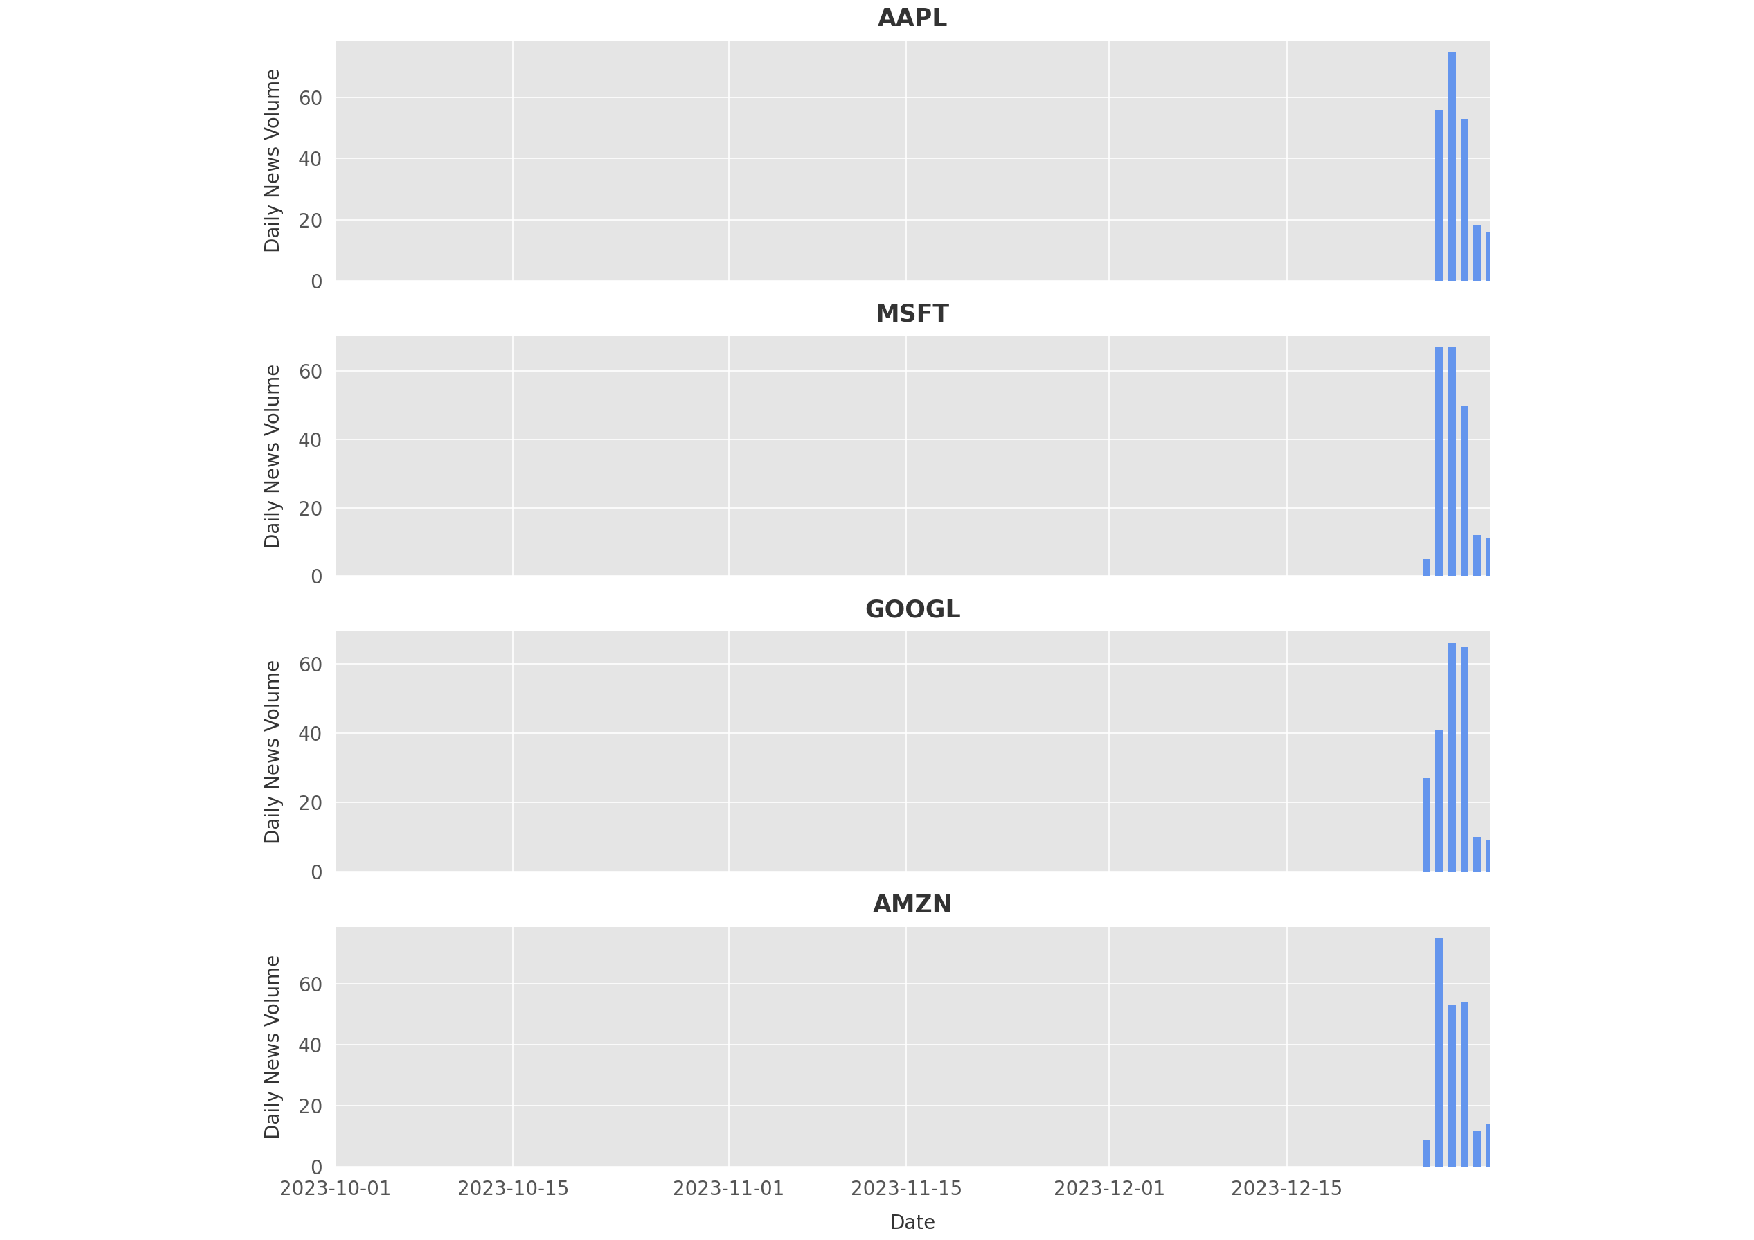
\includegraphics[width=\textwidth]{img/textual-data/q4-2023-a.pdf}
  \caption{Finnhub daily news articles volume of Apple Inc. (AAPL), Microsoft Corp. (MSFT), Alphabet Inc. (GOOGL), and Amazon.com Inc. (AMZN) for the fourth quarter of 2023}
  \label{fig:finnhub-q4-2023}
\end{figure}

\begin{figure}[htbp]
  \centering
  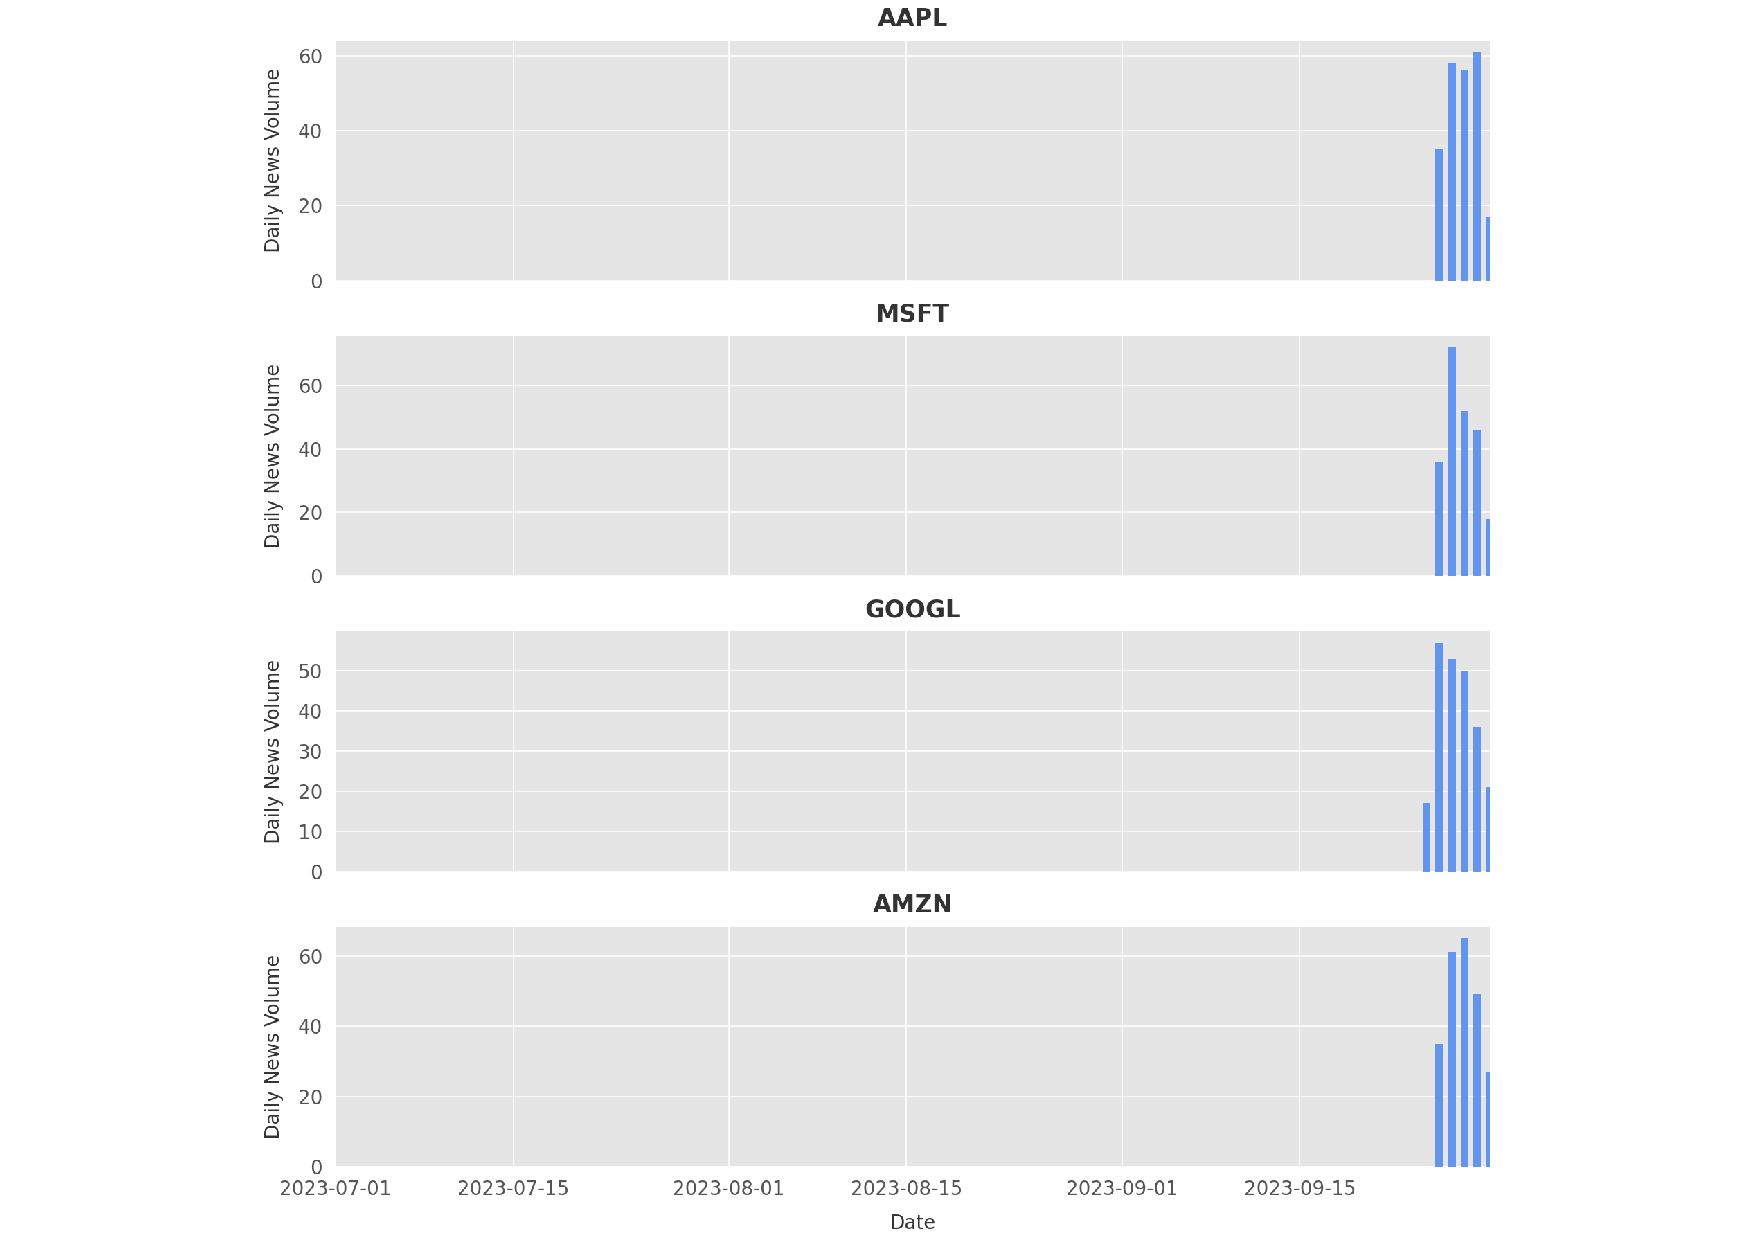
\includegraphics[width=\textwidth]{img/textual-data/q3-2023-a.pdf}
  \caption{Finnhub daily news articles volume of Apple Inc. (AAPL), Microsoft Corp. (MSFT), Alphabet Inc. (GOOGL), and Amazon.com Inc. (AMZN) for the third quarter of 2023}
  \label{fig:finnhub-q3-2023}
\end{figure}

\newpage

\section{First-party Data Providers}
\label{appsec:first-party-data-providers}

\begin{figure}[htbp]
  \centering
  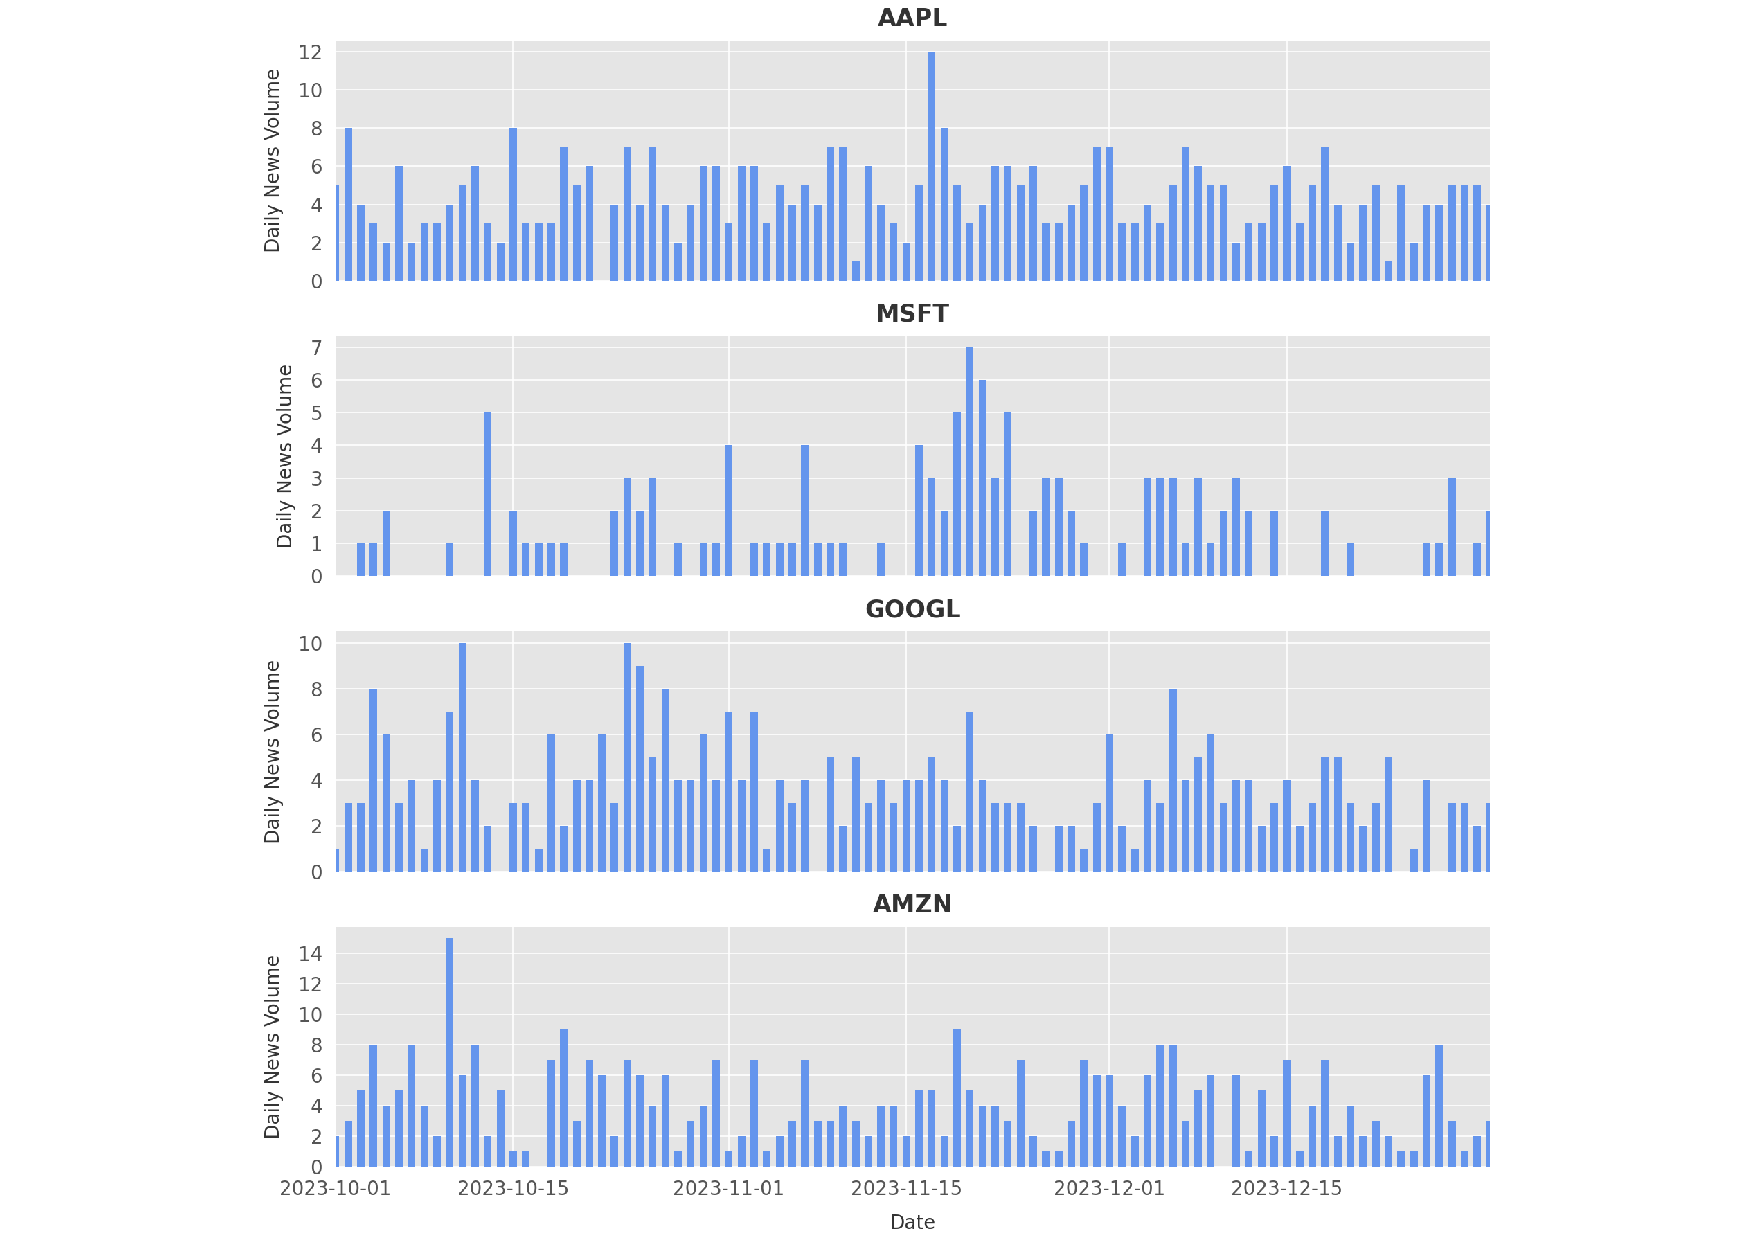
\includegraphics[width=\textwidth]{img/textual-data/guardian-q4-2023-a.pdf}
  \caption{The Guardian daily news articles volume of Apple Inc. (AAPL), Microsoft Corp. (MSFT), Alphabet Inc. (GOOGL), Amazon.com Inc. (AMZN) for the fourth quarter of 2023}
  \label{fig:guardian-q4-2023}
\end{figure}

\begin{figure}[htbp]
  \centering
  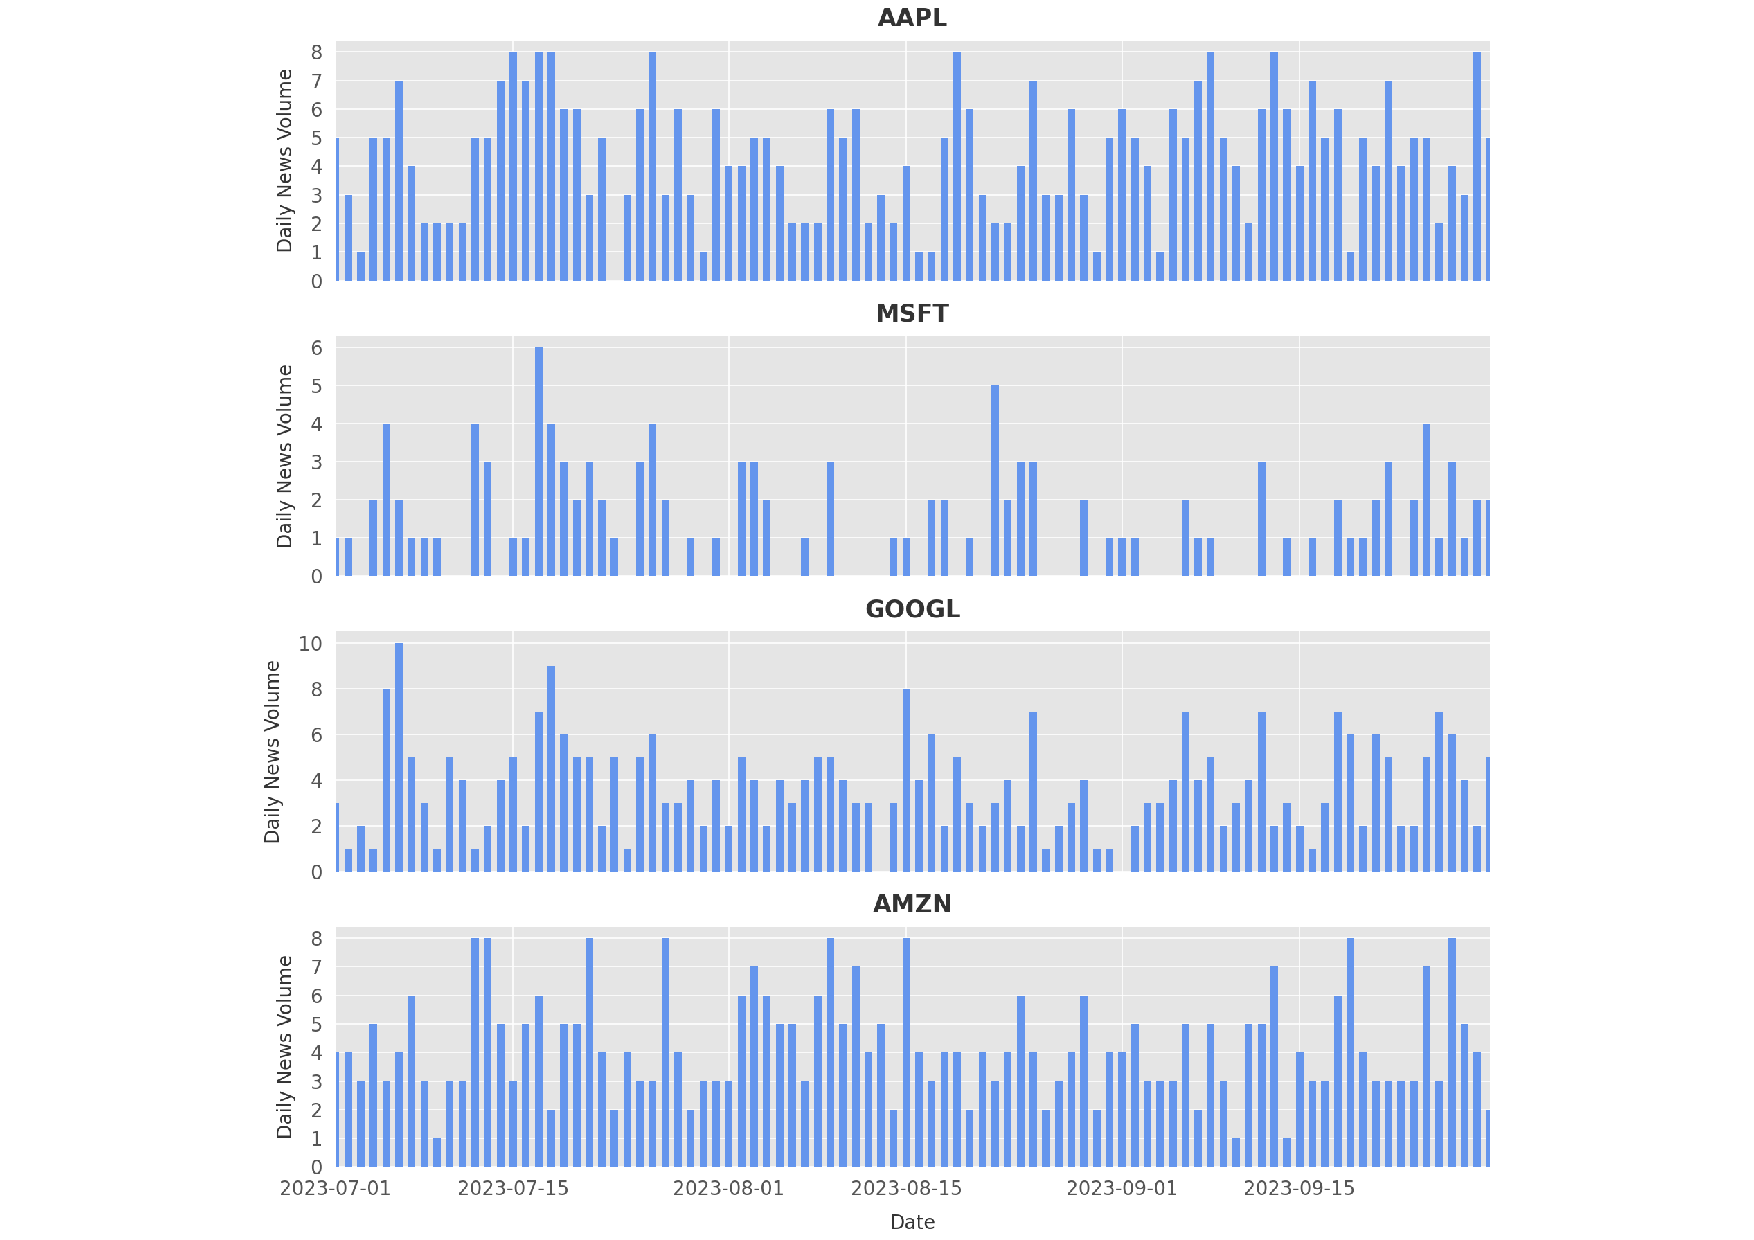
\includegraphics[width=\textwidth]{img/textual-data/guardian-q3-2023-a.pdf}
  \caption{The Guardian daily news articles volume of Apple Inc. (AAPL), Microsoft Corp. (MSFT), Alphabet Inc. (GOOGL), and Amazon.com Inc. (AMZN) for the third quarter of 2023}
  \label{fig:guardian-q3-2023}
\end{figure}

\chapter{SPARQL Wrapper}
\label{app:sparql-wrapper}
This appendix contains the implementation of the SPARQL queries discussed in Section \ref{subsubsec:sparql-wrapper}. The queries are divided into three parts, each representing a different approach to retrieving the ticker symbol of the selected entities. To ensure consistency in the text when comparing results with the naive approach methods, we will refer to the QID (\textit{?id}) and Label (\textit{?idLabel}) related to the Organization entity, as well as Ticker (\textit{?ticker}) and Stock Exchange (\textit{?exchangeLabels}) in the query result tables.

\section{Query 1: Direct ticker retrieval}
\label{appsec:q1-direct-ticker-retrieval}

\begin{lstlisting}[language=SPARQL, caption={SPARQL Query 1: Retrieve entity information for entities directly with the \textit{stock exchange} property.}, label={lst:sparql_query_1}]
    SELECT DISTINCT 
      ?id             # Selects the entity ID
      ?idLabel        # Selects the label of the entity
      ?exchangesLabel # Selects the label of the exchange
      ?ticker         # Selects the ticker symbol
    
    WHERE {
      # Retrieves labels in English
      SERVICE wikibase:label {
        bd:serviceParam wikibase:language 
            "[AUTO_LANGUAGE],en".
      }
    
      # Specifies the QIDs of the entities
      VALUES ?id { 
        wd:Q11463    # Adobe
        wd:Q3884     # Amazon
        wd:Q95       # Google
        wd:Q37156    # IBM
        wd:Q18811574 # Meta
        wd:Q2283     # Microsoft
        wd:Q48938223 # TikTok
        wd:Q21708200 # OpenAI
        wd:Q209330   # Instagram
      }
    
      # Specifies the QIDs of the stock exchanges
      VALUES ?exchanges { 
        wd:Q82059    # NASDAQ
        wd:Q13677    # NYSE
      }
    
      # Matches entities with stock exchange property
      ?id p:P414 ?exchange.
    
      # Filters the exchanges to those specified 
      # and retrieves the ticker symbol
      ?exchange ps:P414 ?exchanges; 
               pq:P249 ?ticker.

      # Filters tickers without an end time
      FILTER NOT EXISTS {
          ?exchange pq:P582 ?endTime.
      }
    }
\end{lstlisting}

\section{Query 2: Owner-based ticker retrieval}
\label{appsec:q2-owner-based-ticker-retrieval}

\begin{lstlisting}[language=SPARQL, caption={SPARQL Query 2: Retrieve entity information for remaining entities with the \textit{owned by} property.}, label={lst:sparql_query_2}]
    SELECT DISTINCT 
      ?id             # Selects the entity ID
      ?idLabel        # Selects the label of the entity
      ?exchangesLabel # Selects the label of the exchange
      ?ticker         # Selects the ticker symbol
      
    WHERE {
      # Retrieves labels in English
      SERVICE wikibase:label {
        bd:serviceParam wikibase:language 
            "[AUTO_LANGUAGE],en".
      }
    
      # Specifies the QIDs of the remaining entities
      VALUES ?id { 
        wd:Q95       # Google
        wd:Q18811574 # Meta
        wd:Q48938223 # TikTok
        wd:Q21708200 # OpenAI
        wd:Q209330   # Instagram        
       }
    
      # Specifies the QIDs of the stock exchanges
      VALUES ?exchanges { 
        wd:Q82059    # NASDAQ
        wd:Q13677    # NYSE
      }
    
      # Matches entities with owner property
      ?id wdt:P127 ?owner.
      ?owner p:P414 ?exchange.
    
      # Filters the exchanges to those specified 
      # and retrieves the ticker symbol
      ?exchange ps:P414 ?exchanges; 
               pq:P249 ?ticker.

      # Filters tickers without an end time
      FILTER NOT EXISTS {
          ?exchange pq:P582 ?endTime.
      }
    }
\end{lstlisting}

\section{Query 3: Differentiated ticker retrieval}
\label{appsec:q3-differentiated-ticker-retrieval}

\begin{lstlisting}[language=SPARQL, caption={SPARQL Query 3: Retrieve entity information for remaining entities with the \textit{different from} property.}, label={lst:sparql_query_3}]
	SELECT DISTINCT 
	  ?id             # Selects the entity ID
	  ?idLabel        # Selects the label of the entity
	  ?exchangesLabel # Selects the label of the exchange
	  ?ticker         # Selects the ticker symbol
	  
	WHERE {
	  # Retrieves labels in English
	  SERVICE wikibase:label {
		bd:serviceParam wikibase:language 
			"[AUTO_LANGUAGE],en".
	  }
	
	  # Specifies the QIDs of the remaining entities
	  VALUES ?id { 
		wd:Q18811574 # Meta
		wd:Q48938223 # TikTok
		wd:Q21708200 # OpenAI
	  }
	
	  # Specifies the QIDs of the stock exchanges
	  VALUES ?exchanges { 
		wd:Q82059    # NASDAQ
		wd:Q13677    # NYSE
	  }
	
	  # Matches entities with the 'different from' property
	  ?id wdt:P1889 ?differs.
	  ?differs p:P414 ?exchange.
	
	  # Filters the exchanges to those specified 
	  # and retrieves the ticker symbol
	  ?exchange ps:P414 ?exchanges; 
			   pq:P249 ?ticker.
			   
	  # Filters tickers without an end time
	  FILTER NOT EXISTS {
		  ?exchange pq:P582 ?endTime.
	  }
	}
  \end{lstlisting}

\chapter{Sentiment and Adjusted Close Price}
\label{app:sentiment-adjusted-close-price}
This appendix presents the outcomes of the sentiment based hold strategy outlined in Section \ref{subsec:elsa-hold-strategy}, along with the analysis of the correlation between sentiment and the adjusted close prices of selected companies, as detailed in Section \ref{subsec:elsa-correlation}.

\section{Hold Strategy}
\label{appsec:hold-strategy}

\begin{figure}[ht]
  \centering
  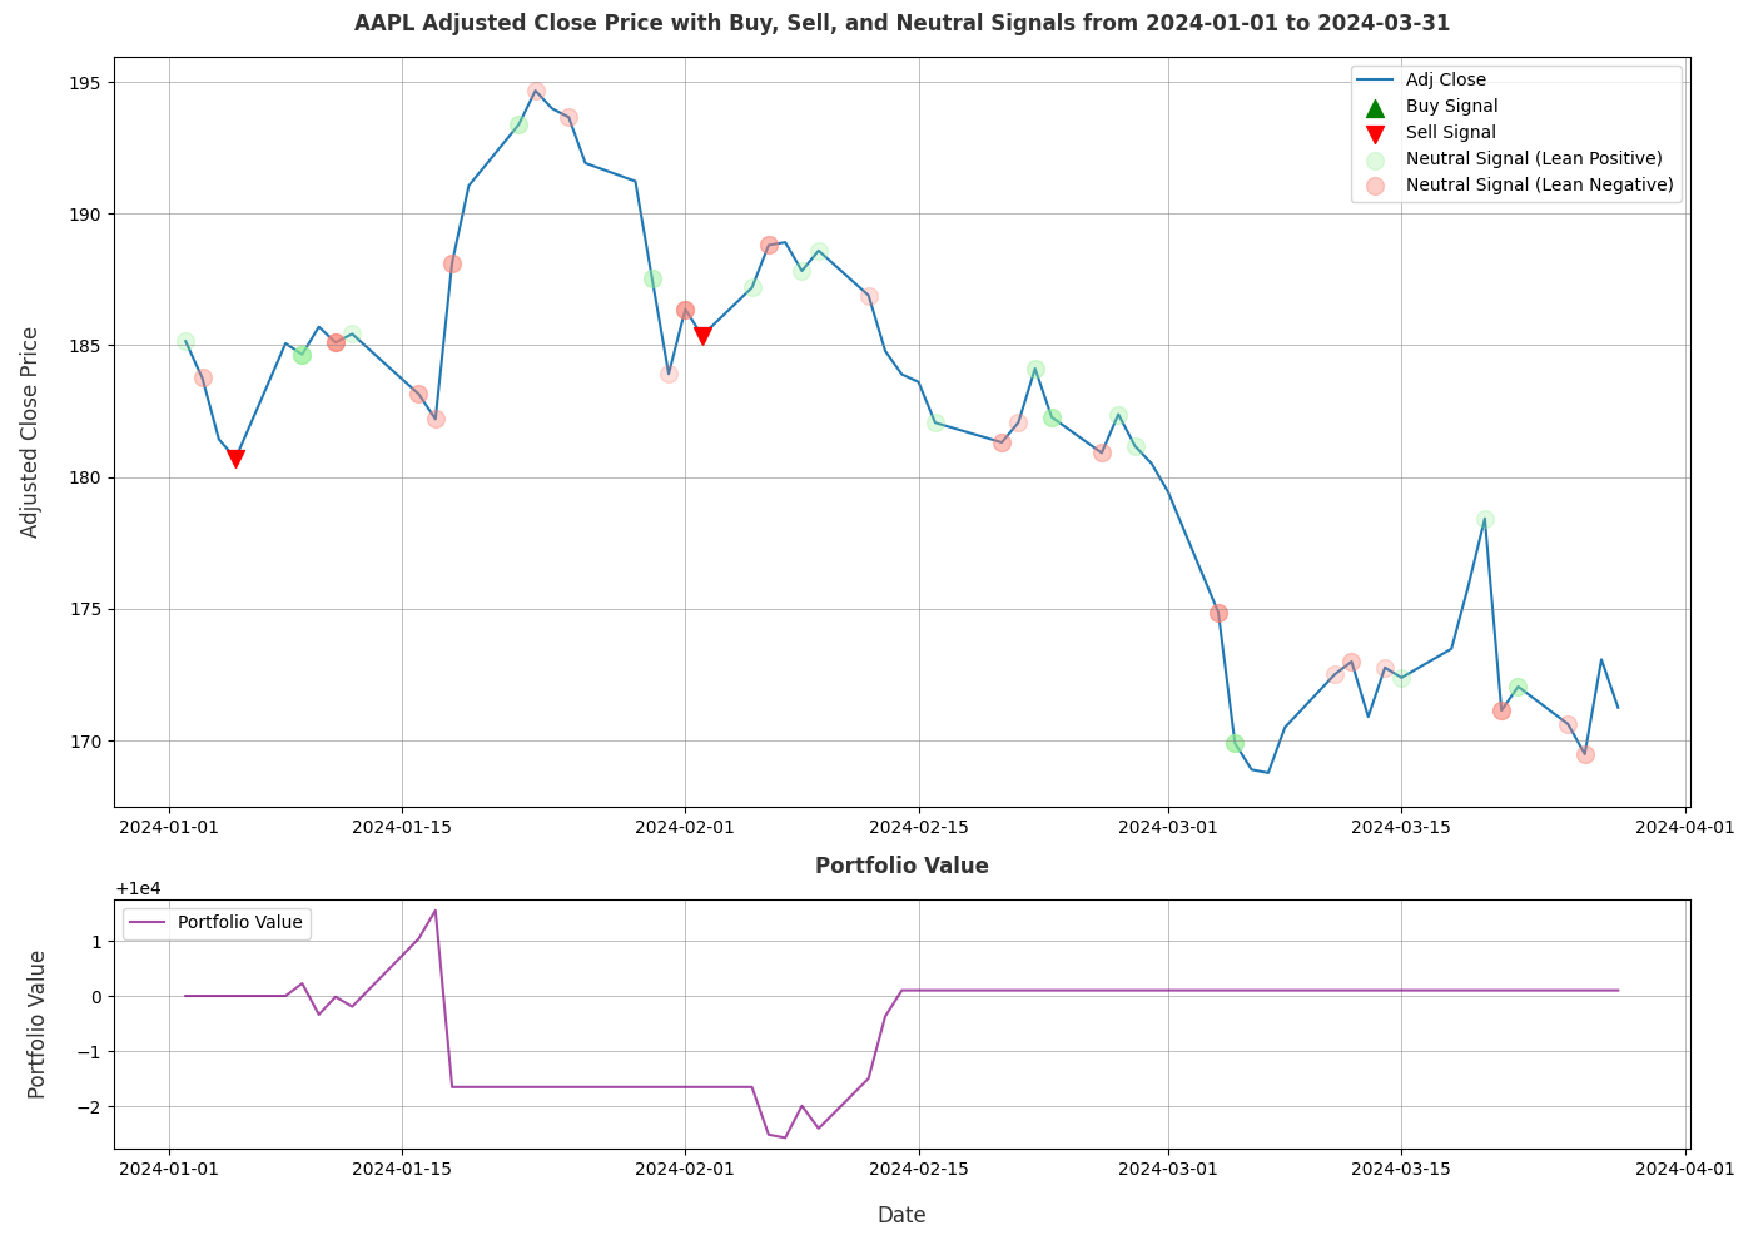
\includegraphics[width=0.9\textwidth]{img/experiment-stock/aapl-hold-strategy-neutral-a.pdf}
  \caption{Apple Inc. (AAPL) adjusted close price with buy, sell and neutral signals in the first quarter of 2024. Hold strategy based on sentiment signals.}
  \label{fig:elsa-experiment-stock-aapl-hold-strategy-neutral}
\end{figure}

\begin{figure}[ht]
  \centering
  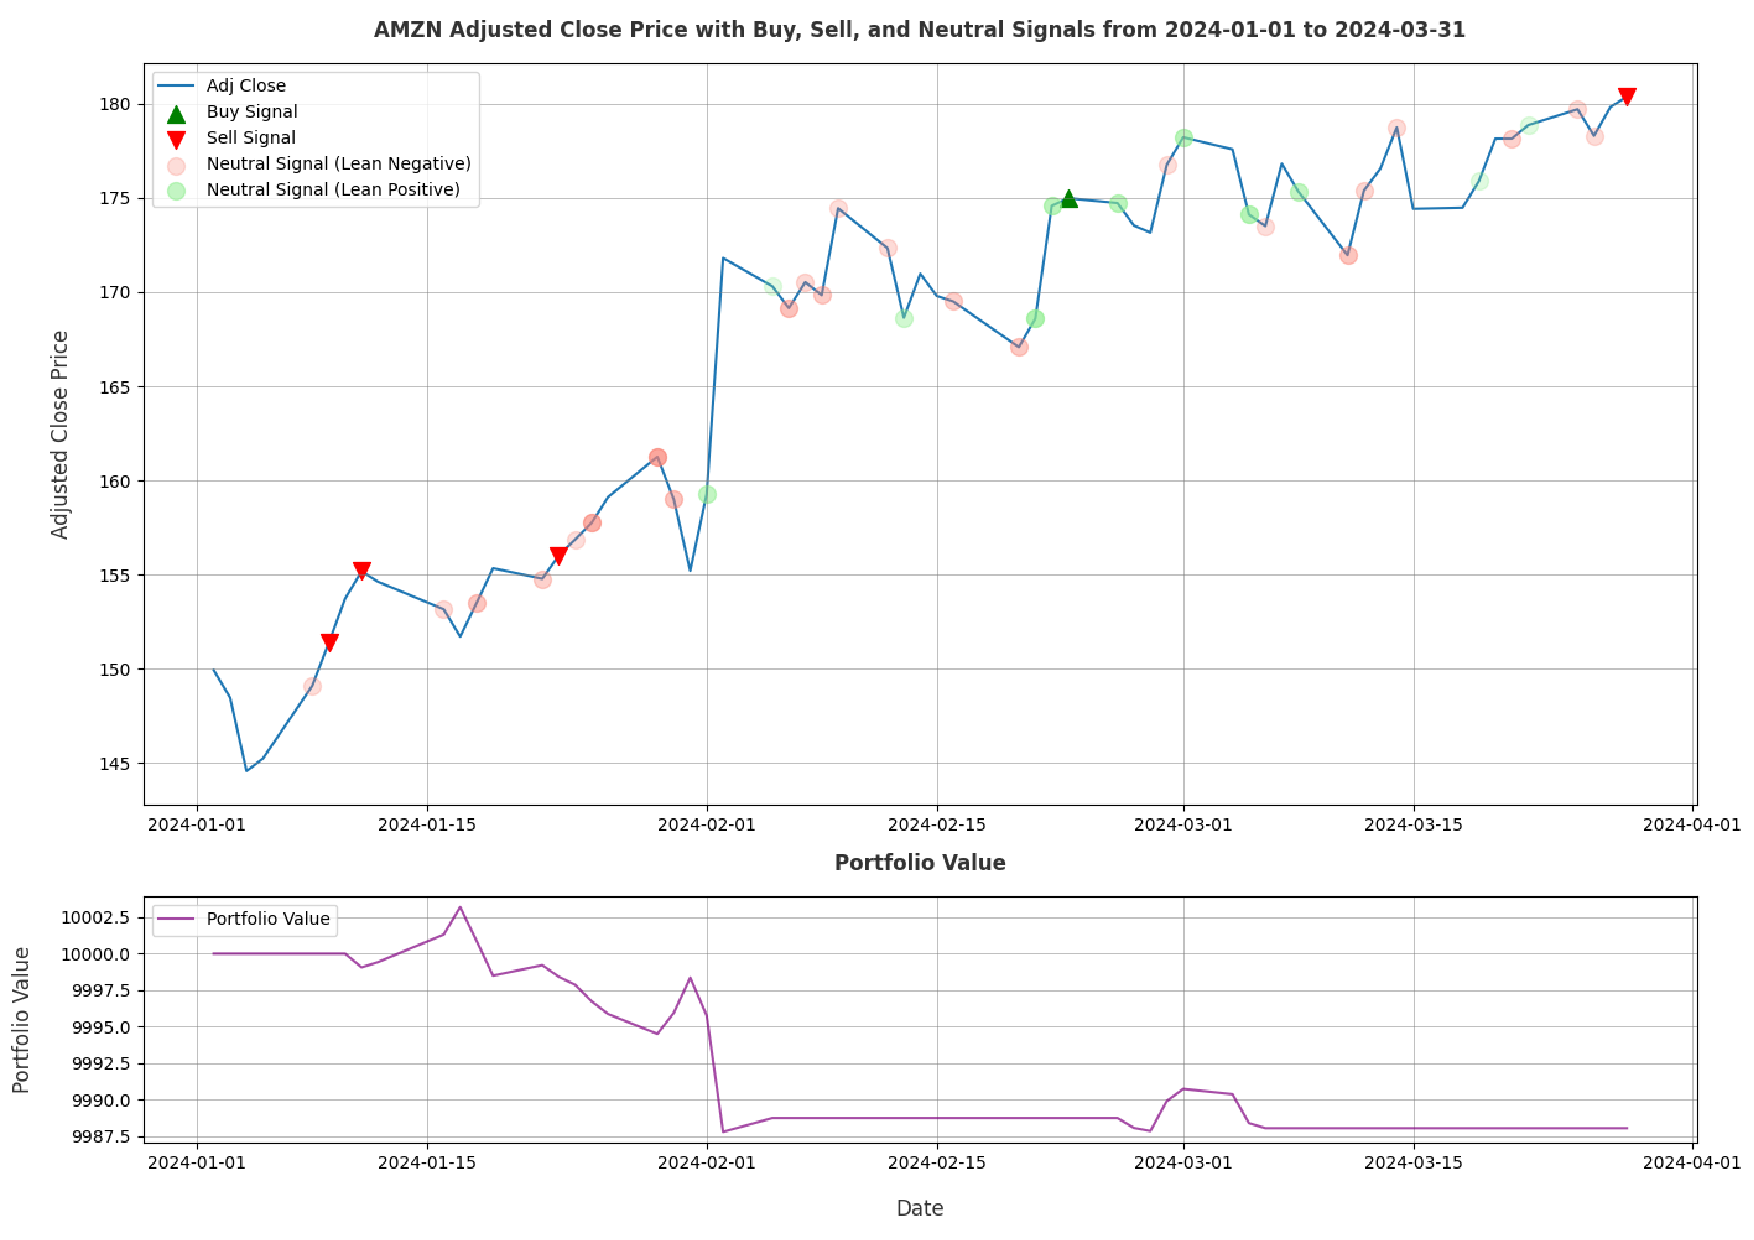
\includegraphics[width=0.9\textwidth]{img/experiment-stock/amzn-hold-strategy-neutral-a.pdf}
  \caption{Amazon.com Inc. (AMZN) adjusted close price with buy, sell and neutral signals in the first quarter of 2024. Hold strategy based on sentiment signals.}
  \label{fig:elsa-experiment-stock-amzn-hold-strategy-neutral}
\end{figure}

\begin{figure}[ht]
  \centering
  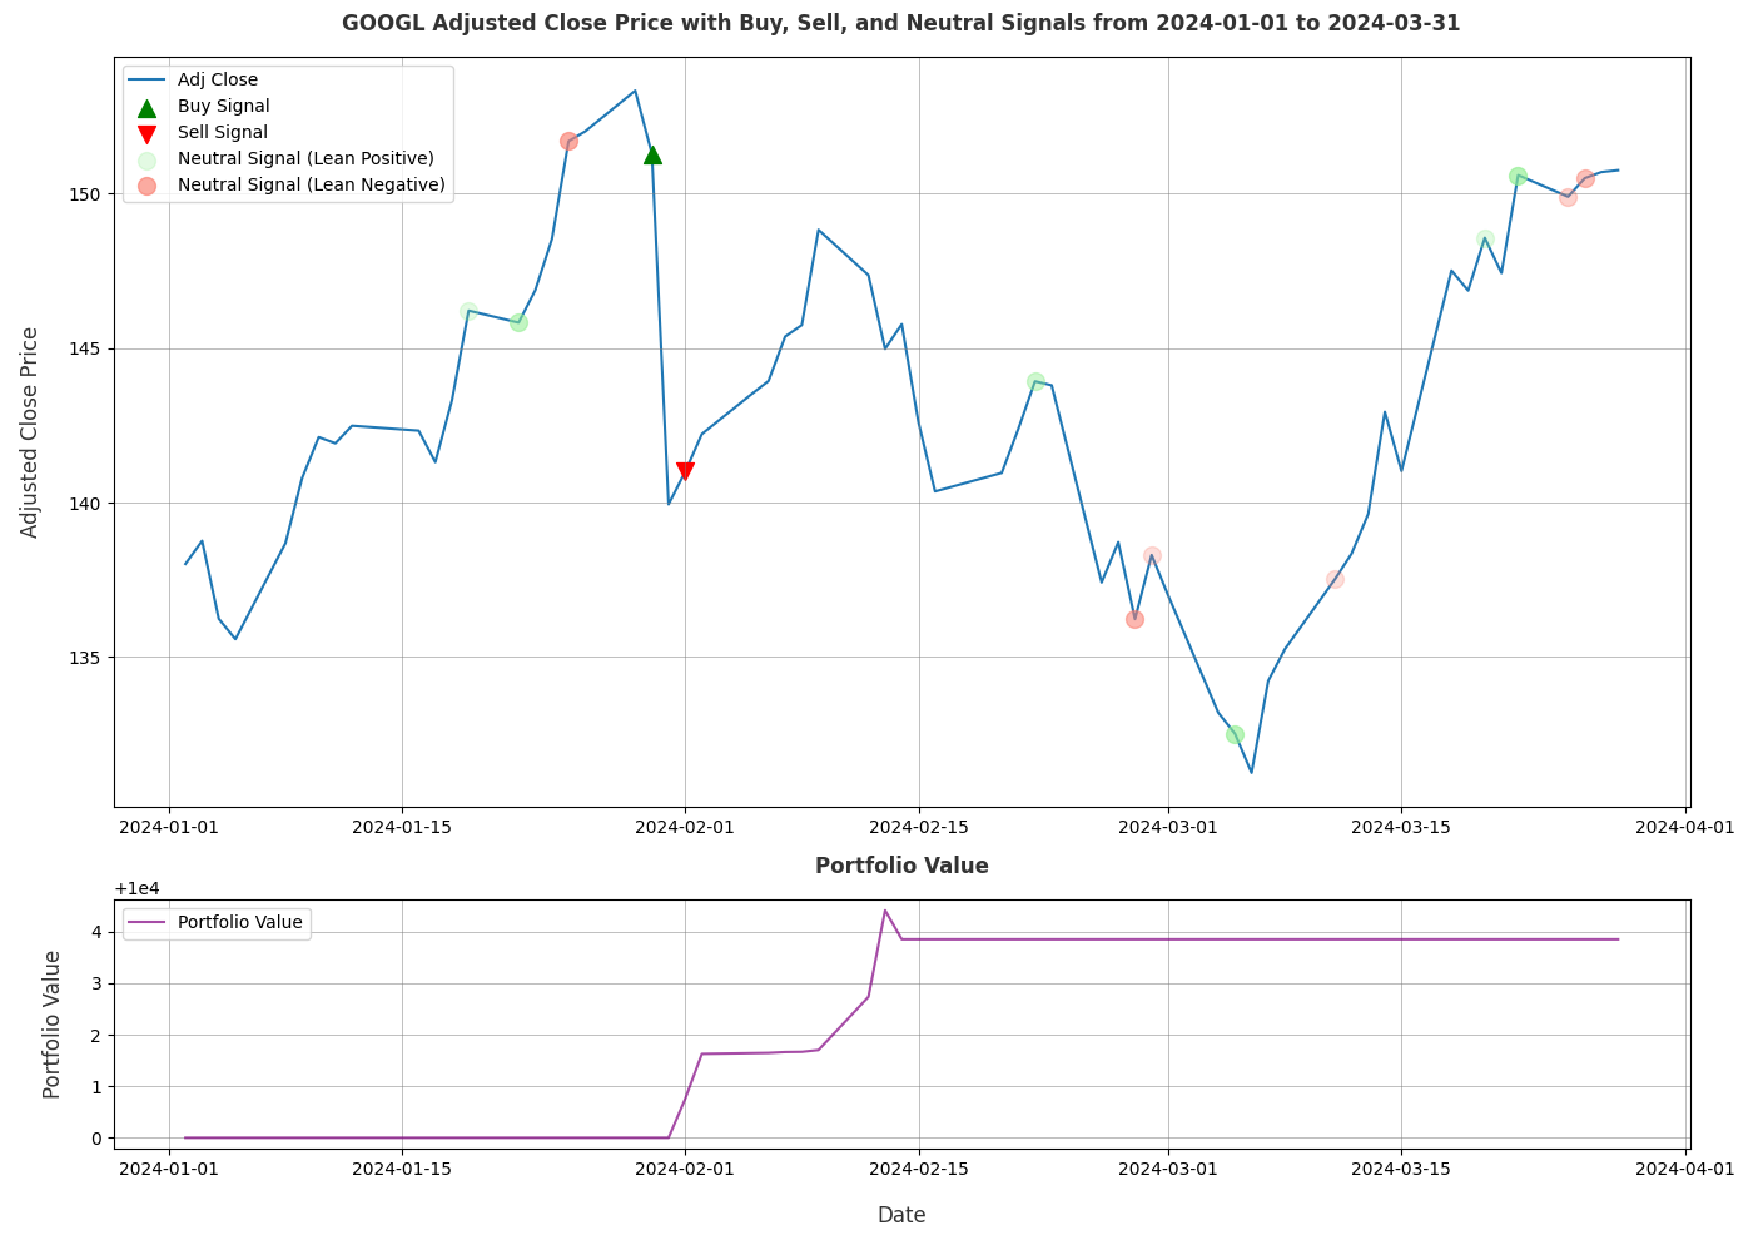
\includegraphics[width=0.9\textwidth]{img/experiment-stock/googl-hold-strategy-neutral-a.pdf}
  \caption{Alphabet Inc. (GOOGL) adjusted close price with buy, sell and neutral signals in the first quarter of 2024. Hold strategy based on sentiment signals.}
  \label{fig:elsa-experiment-stock-googl-hold-strategy-neutral}
\end{figure}

\begin{figure}[ht]
    \centering
    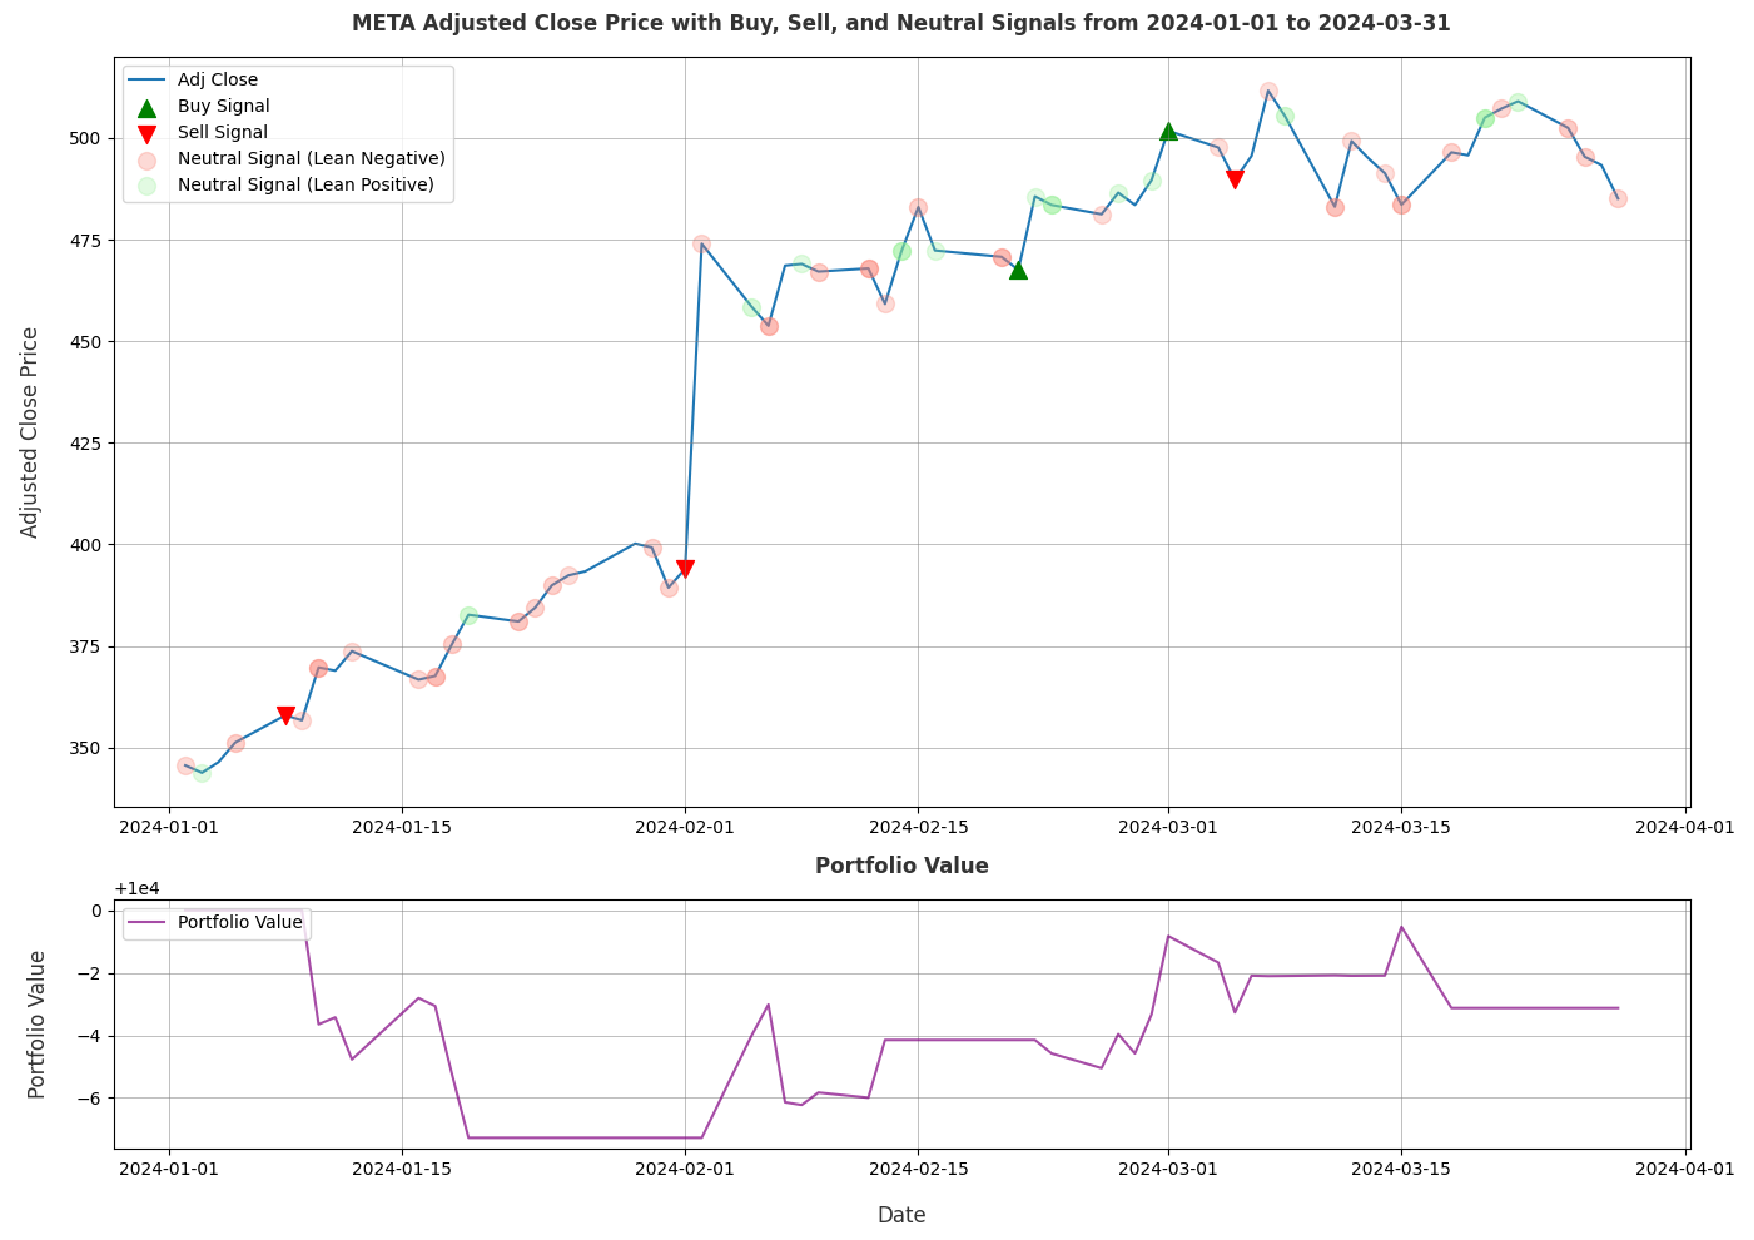
\includegraphics[width=0.9\textwidth]{img/experiment-stock/meta-hold-strategy-neutral-a.pdf}
    \caption{Meta Platforms Inc. (META) adjusted close price with buy, sell and neutral signals in the first quarter of 2024. Hold strategy based on sentiment signals.}
    \label{fig:elsa-experiment-stock-meta-hold-strategy-neutral}
\end{figure}

\begin{figure}[ht]
  \centering
  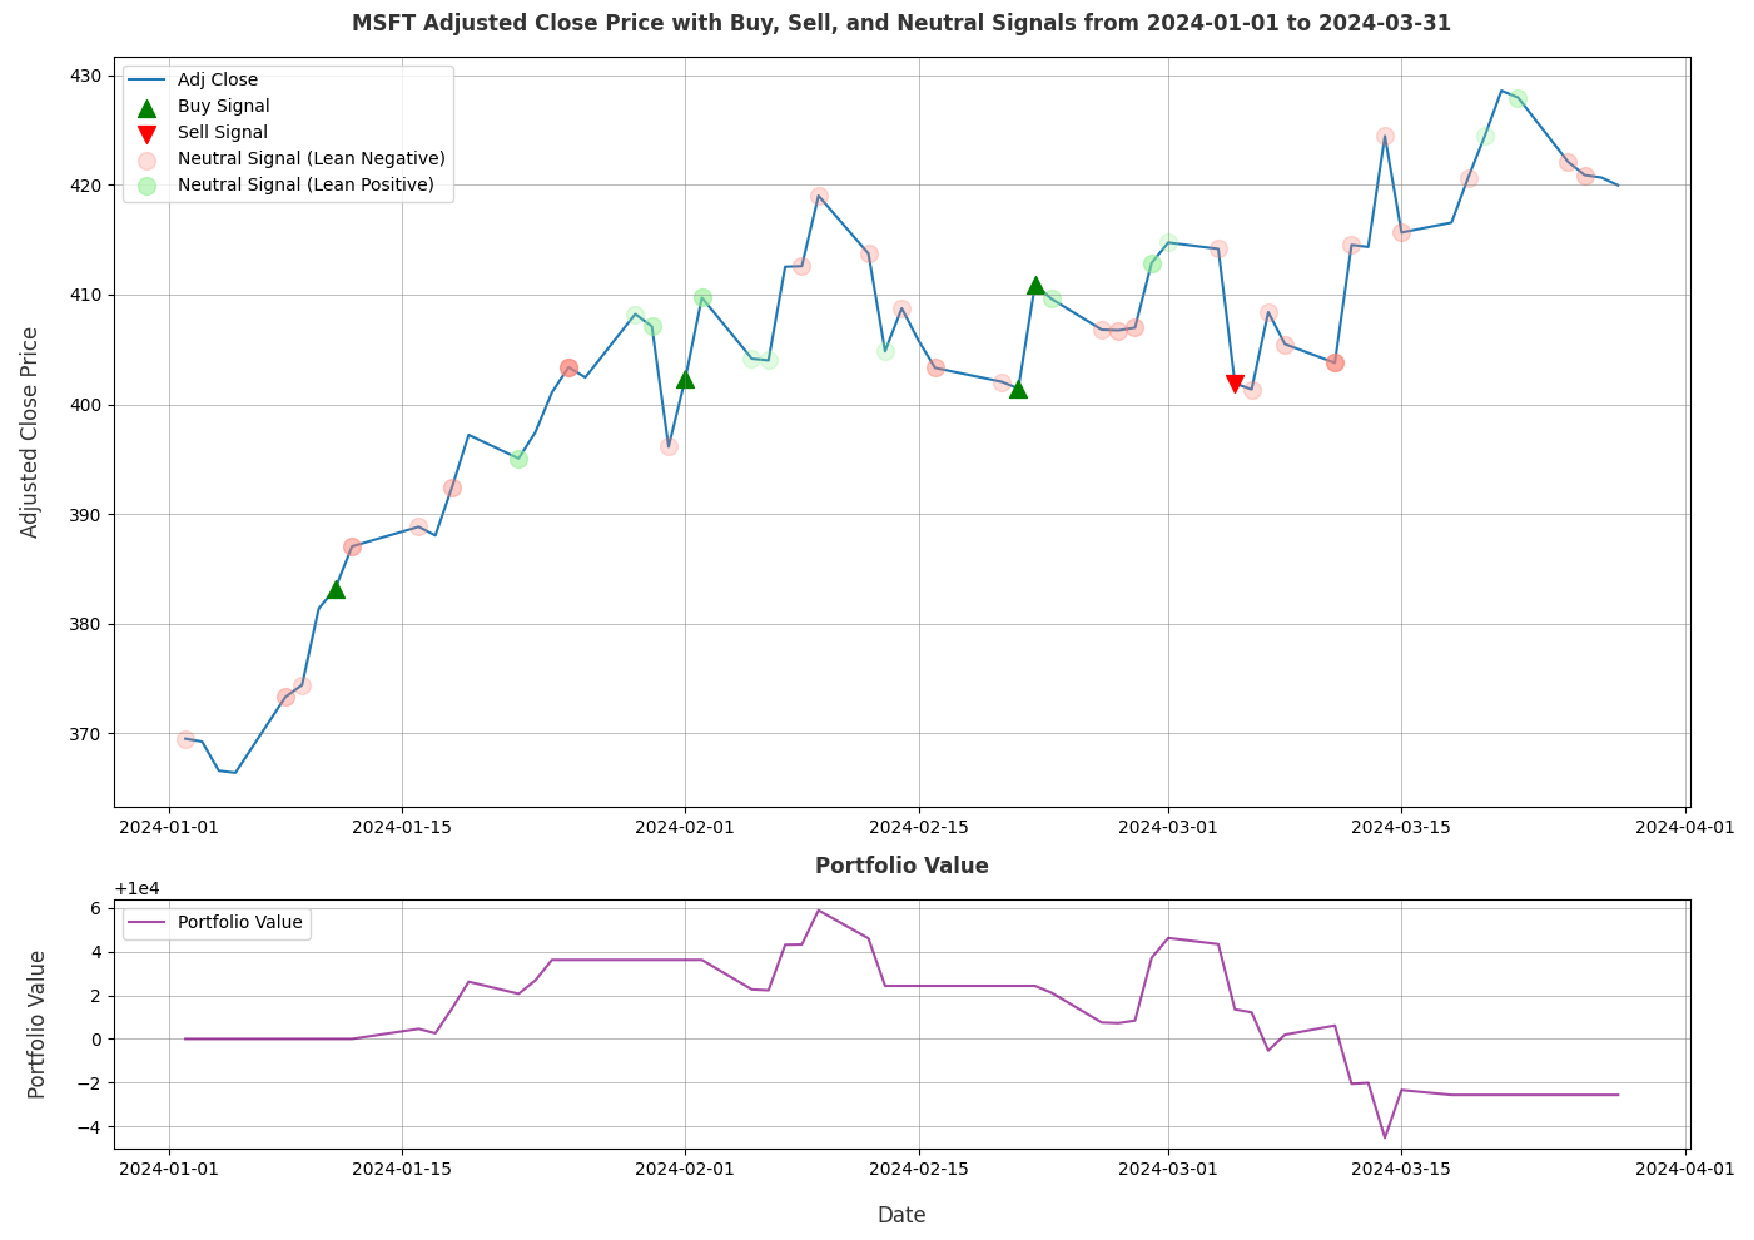
\includegraphics[width=0.9\textwidth]{img/experiment-stock/msft-hold-strategy-neutral-a.pdf}
  \caption{Microsoft Corp. (MSFT) adjusted close price with buy, sell and neutral signals in the first quarter of 2024. Hold strategy based on sentiment signals.}
  \label{fig:elsa-experiment-stock-msft-hold-strategy-neutral}
\end{figure}

\clearpage
\begin{figure}[ht]
  \centering
  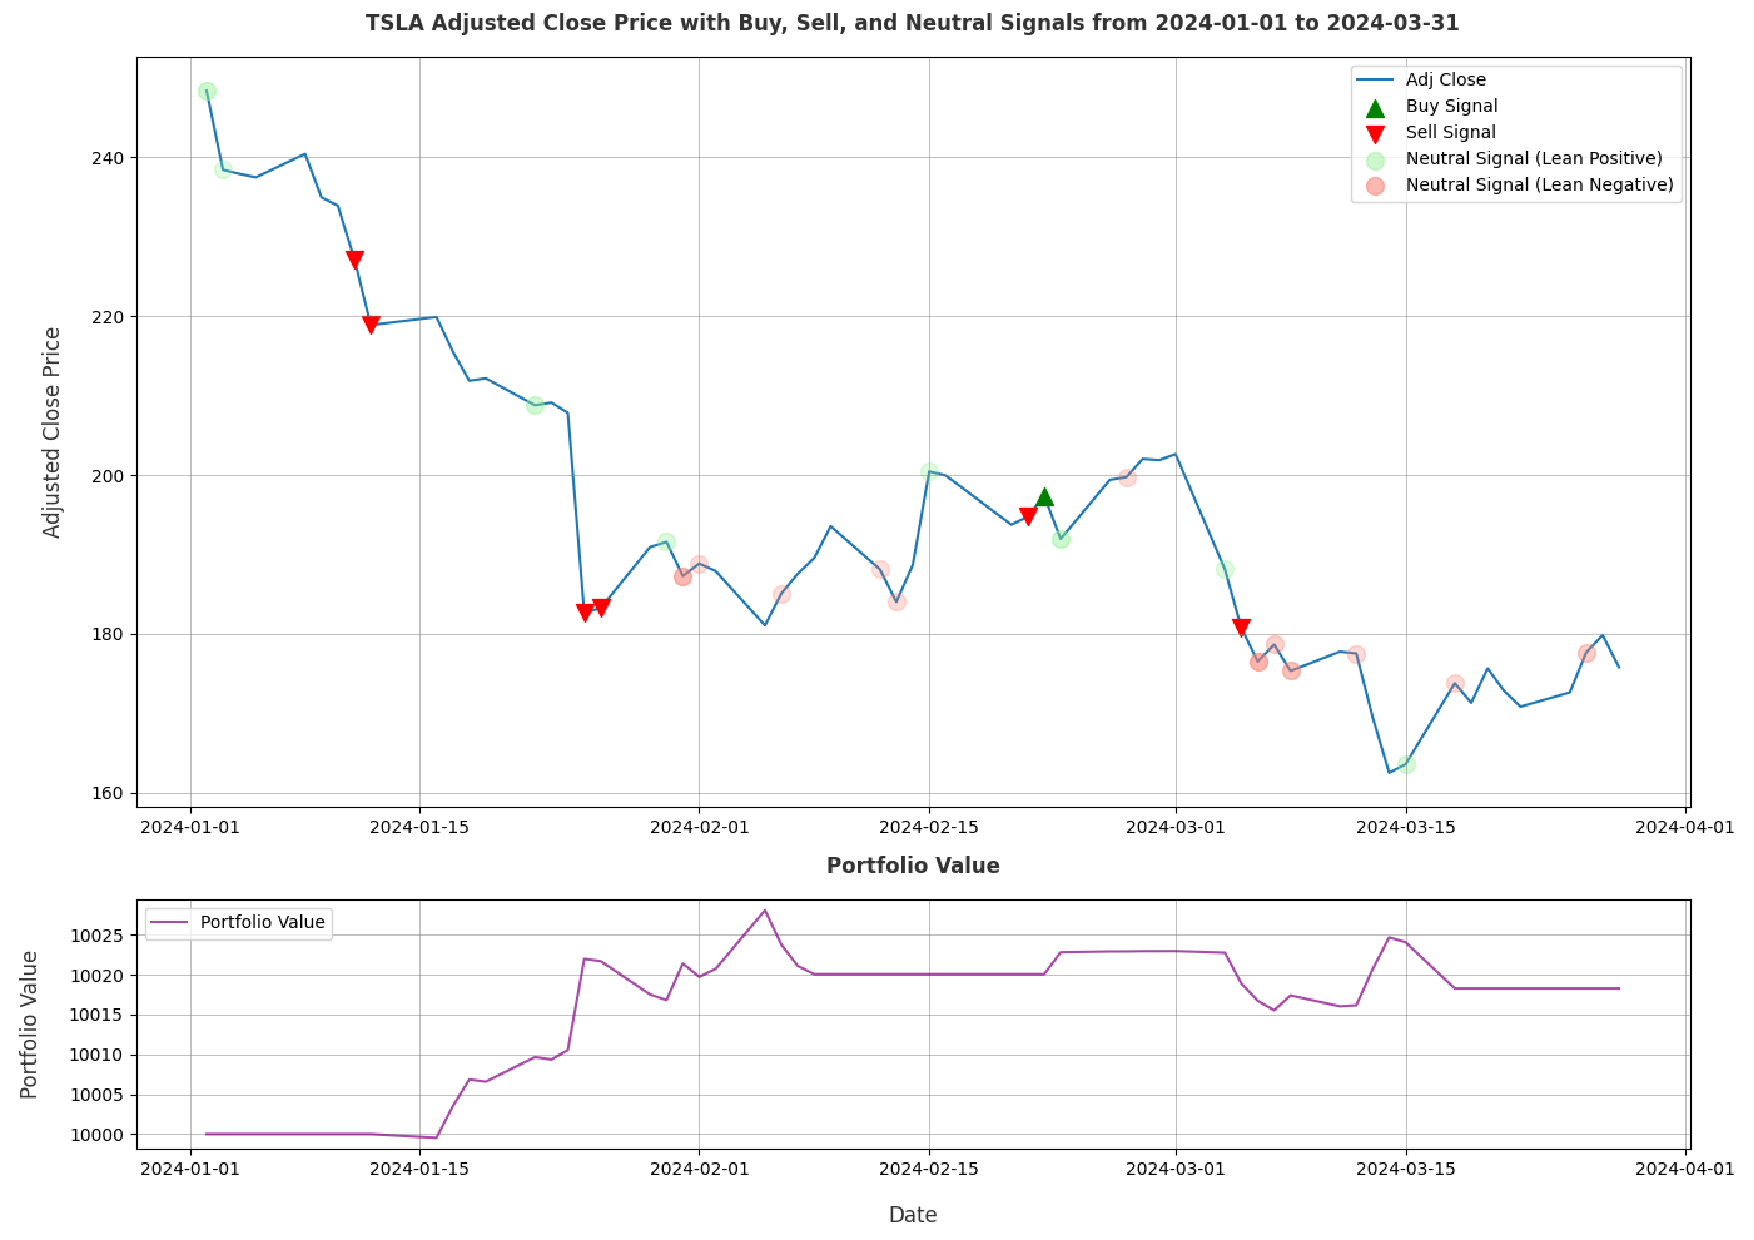
\includegraphics[width=0.9\textwidth]{img/experiment-stock/tsla-hold-strategy-neutral-a.pdf}
  \caption{Tesla Inc. (TSLA) adjusted close price with buy, sell and neutral signals in the first quarter of 2024. Hold strategy based on sentiment signals.}
  \label{fig:elsa-experiment-stock-tsla-hold-strategy-neutral}
\end{figure}

\clearpage

\section{Correlation}
\label{appsec:correlation}

\begin{figure}[ht]
  \centering
  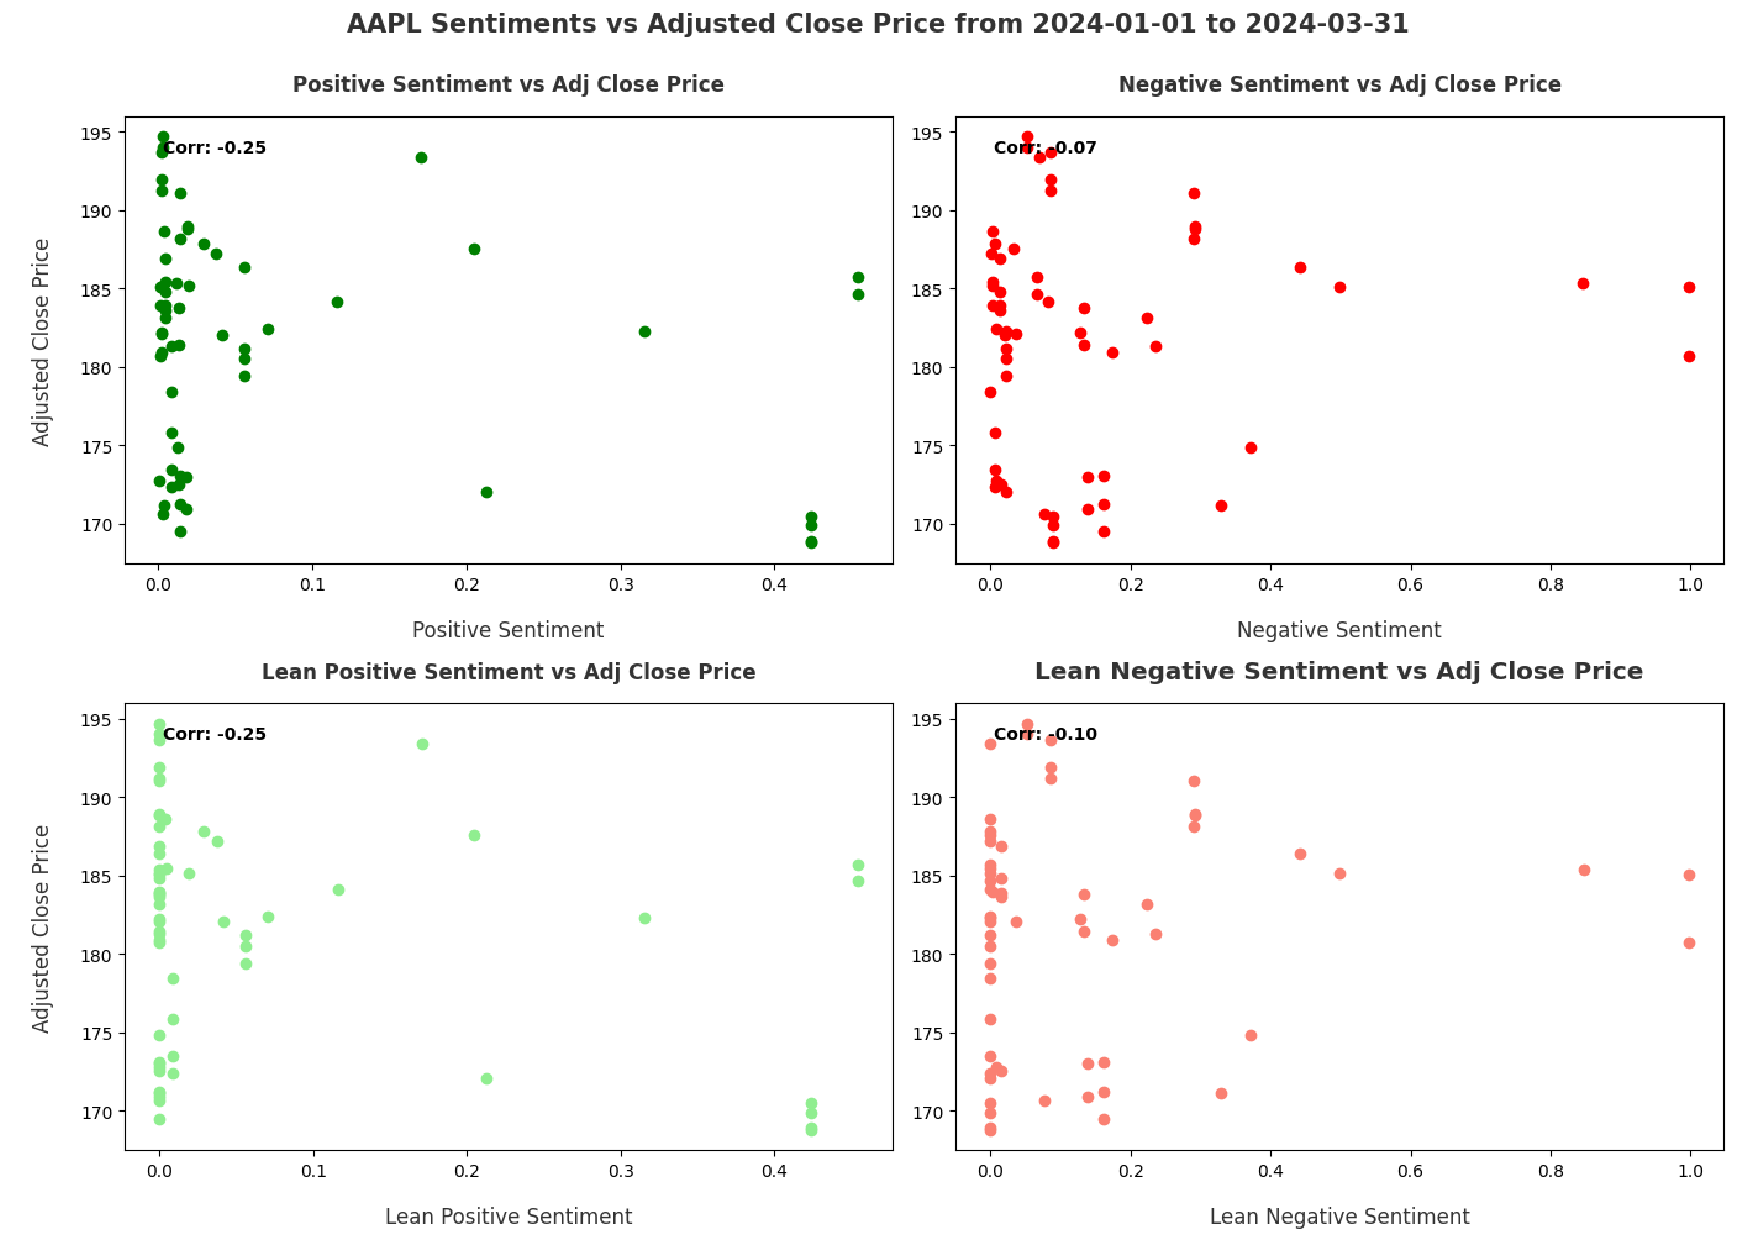
\includegraphics[width=0.9\textwidth]{img/experiment-stock/aapl-corr-a.pdf}
  \caption{Apple Inc. (AAPL) sentiment correlation with adjusted close price in the first quarter of 2024.}
  \label{fig:elsa-experiment-stock-aapl-corr}
\end{figure}

\begin{figure}[htbp]
  \centering
  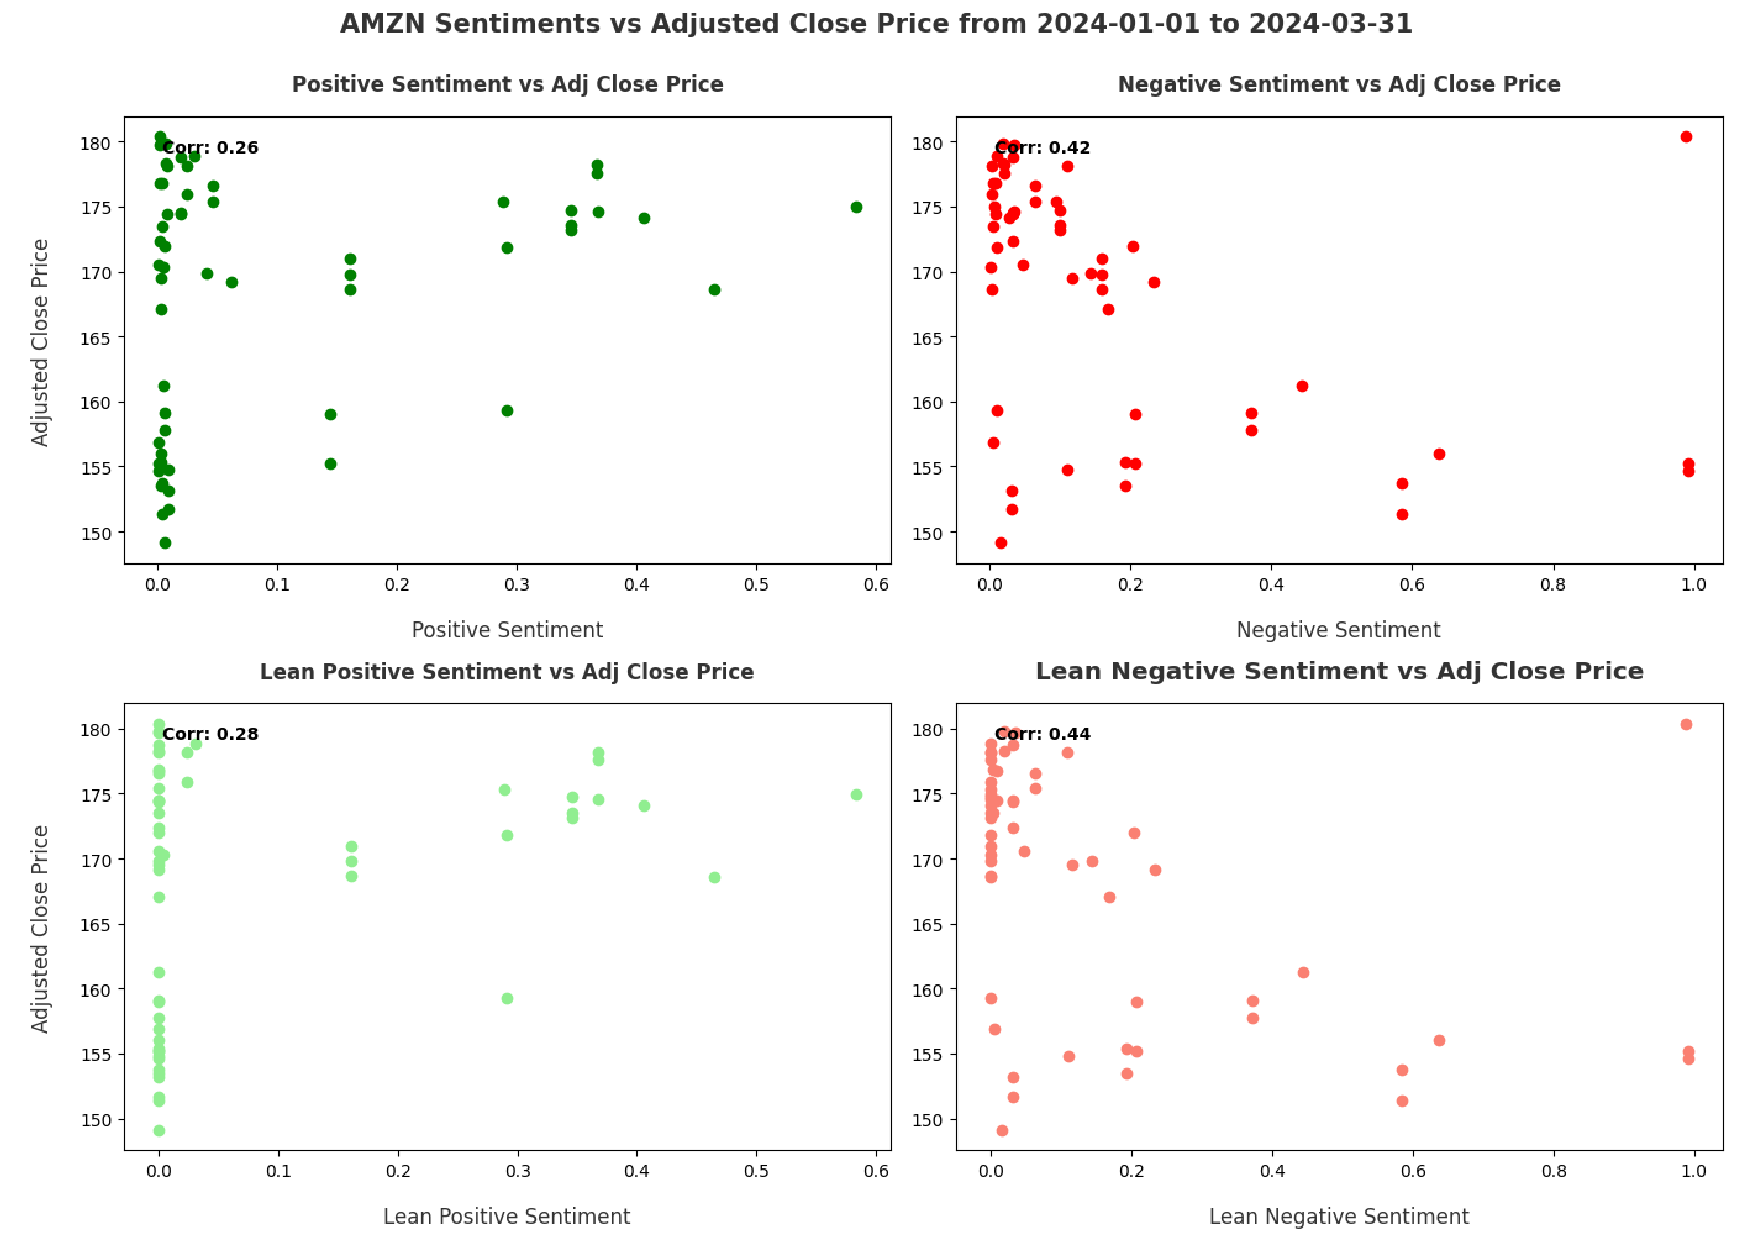
\includegraphics[width=0.9\textwidth]{img/experiment-stock/amzn-corr-a.pdf}
  \caption{Amazon.com Inc. (AMZN) sentiment correlation with adjusted close price in the first quarter of 2024.}
  \label{fig:elsa-experiment-stock-amzn-corr}
\end{figure}

\begin{figure}[htbp]
  \centering
  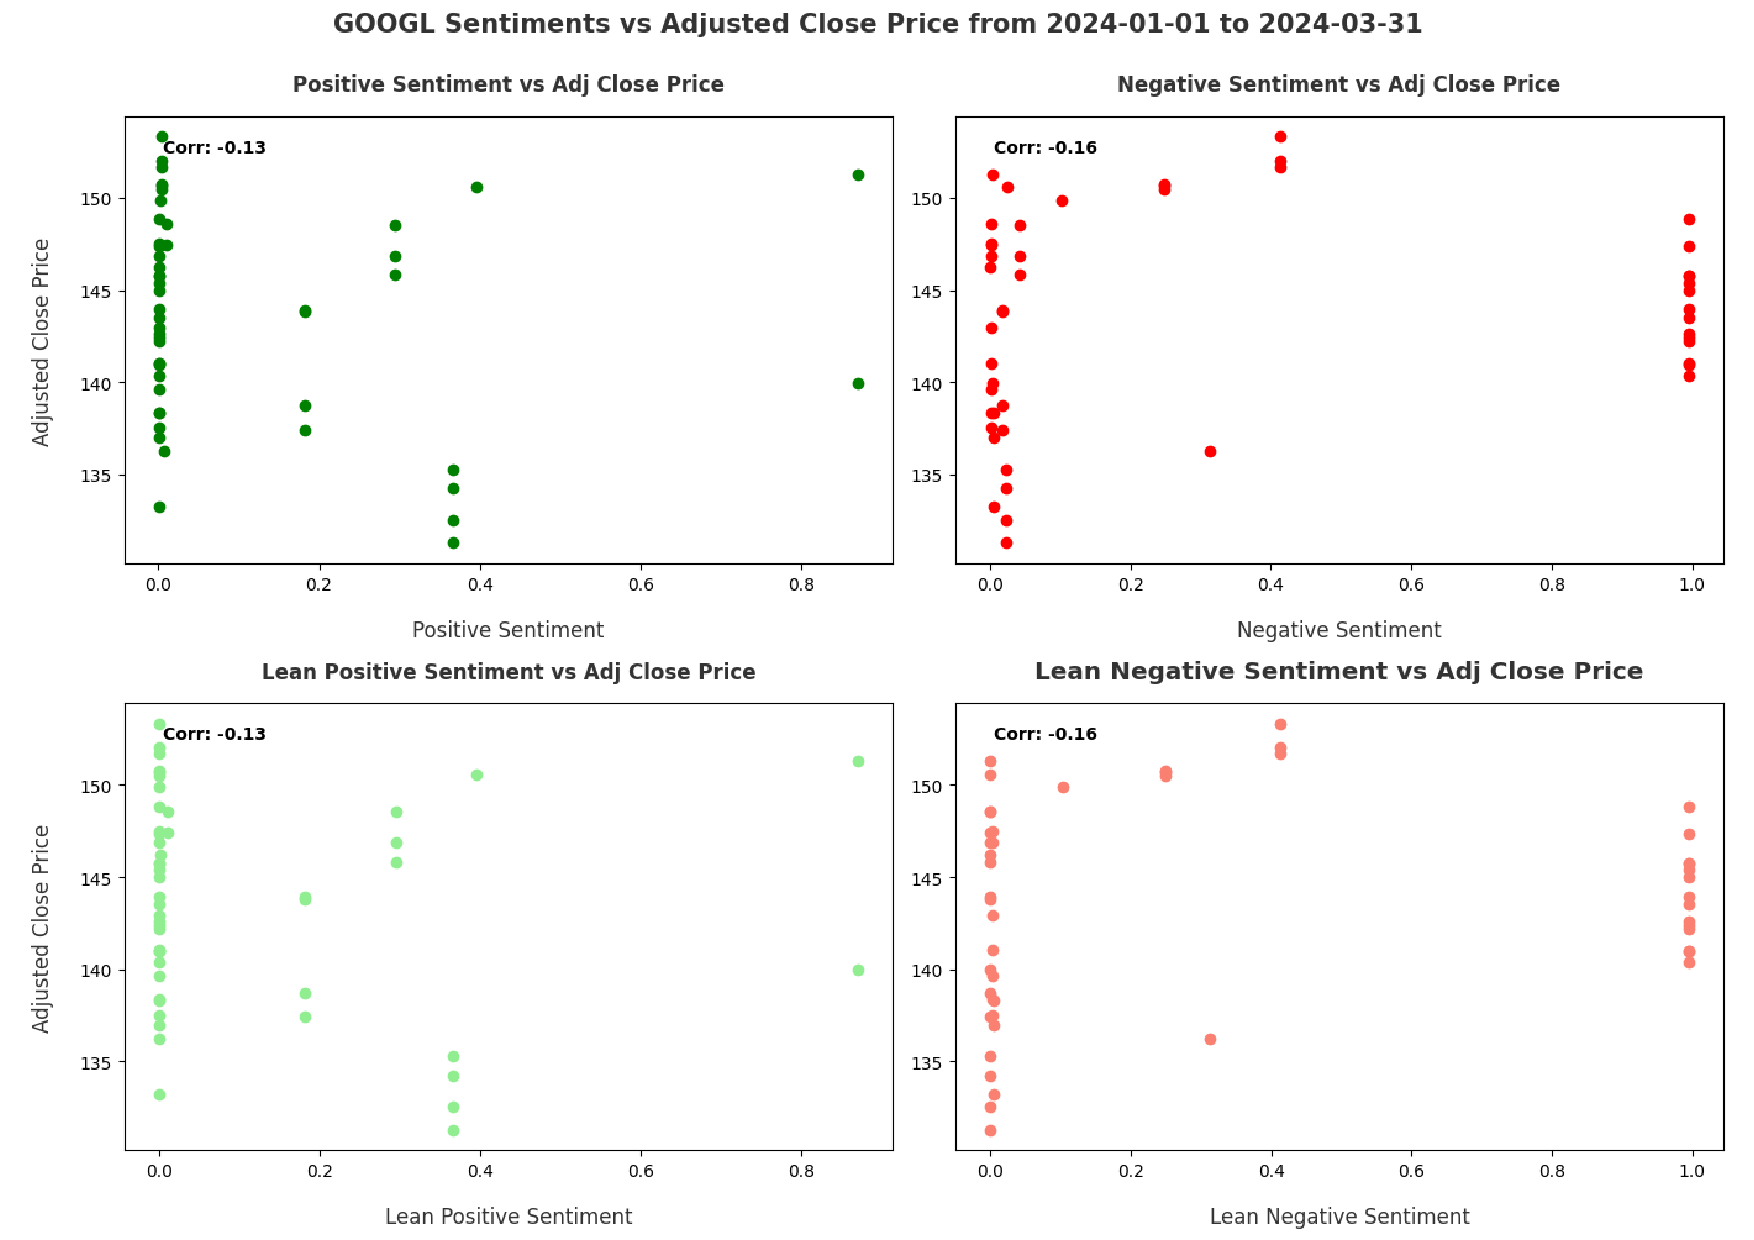
\includegraphics[width=0.9\textwidth]{img/experiment-stock/googl-corr-a.pdf}
  \caption{Alphabet Inc. (GOOGL) sentiment correlation with adjusted close price in the first quarter of 2024.}
  \label{fig:elsa-experiment-stock-googl-corr}
\end{figure}

\begin{figure}[htbp]
    \centering
    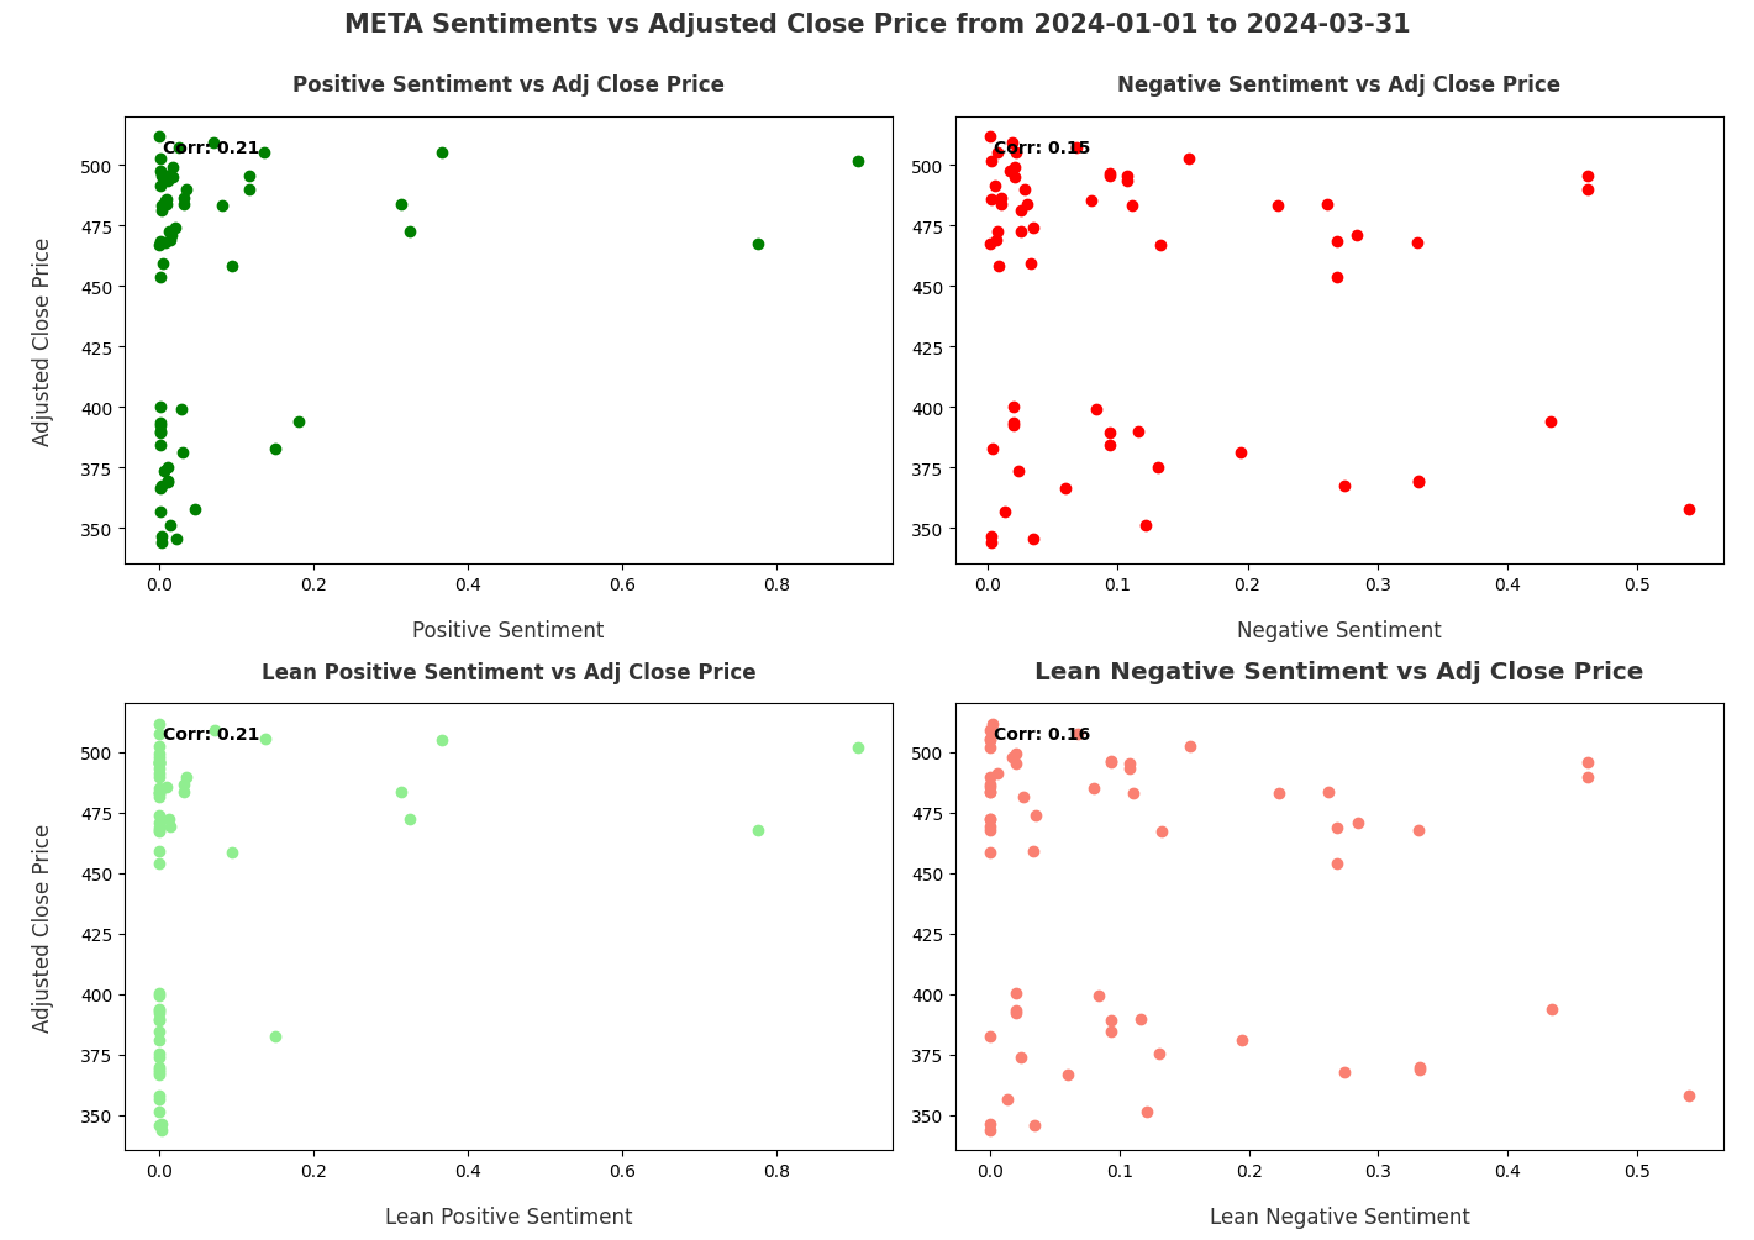
\includegraphics[width=0.9\textwidth]{img/experiment-stock/meta-corr-a.pdf}
    \caption{Meta Platforms Inc. (META) sentiment correlation with adjusted close price in the first quarter of 2024.}
    \label{fig:elsa-experiment-stock-meta-corr}
\end{figure}

\begin{figure}[htbp]
  \centering
  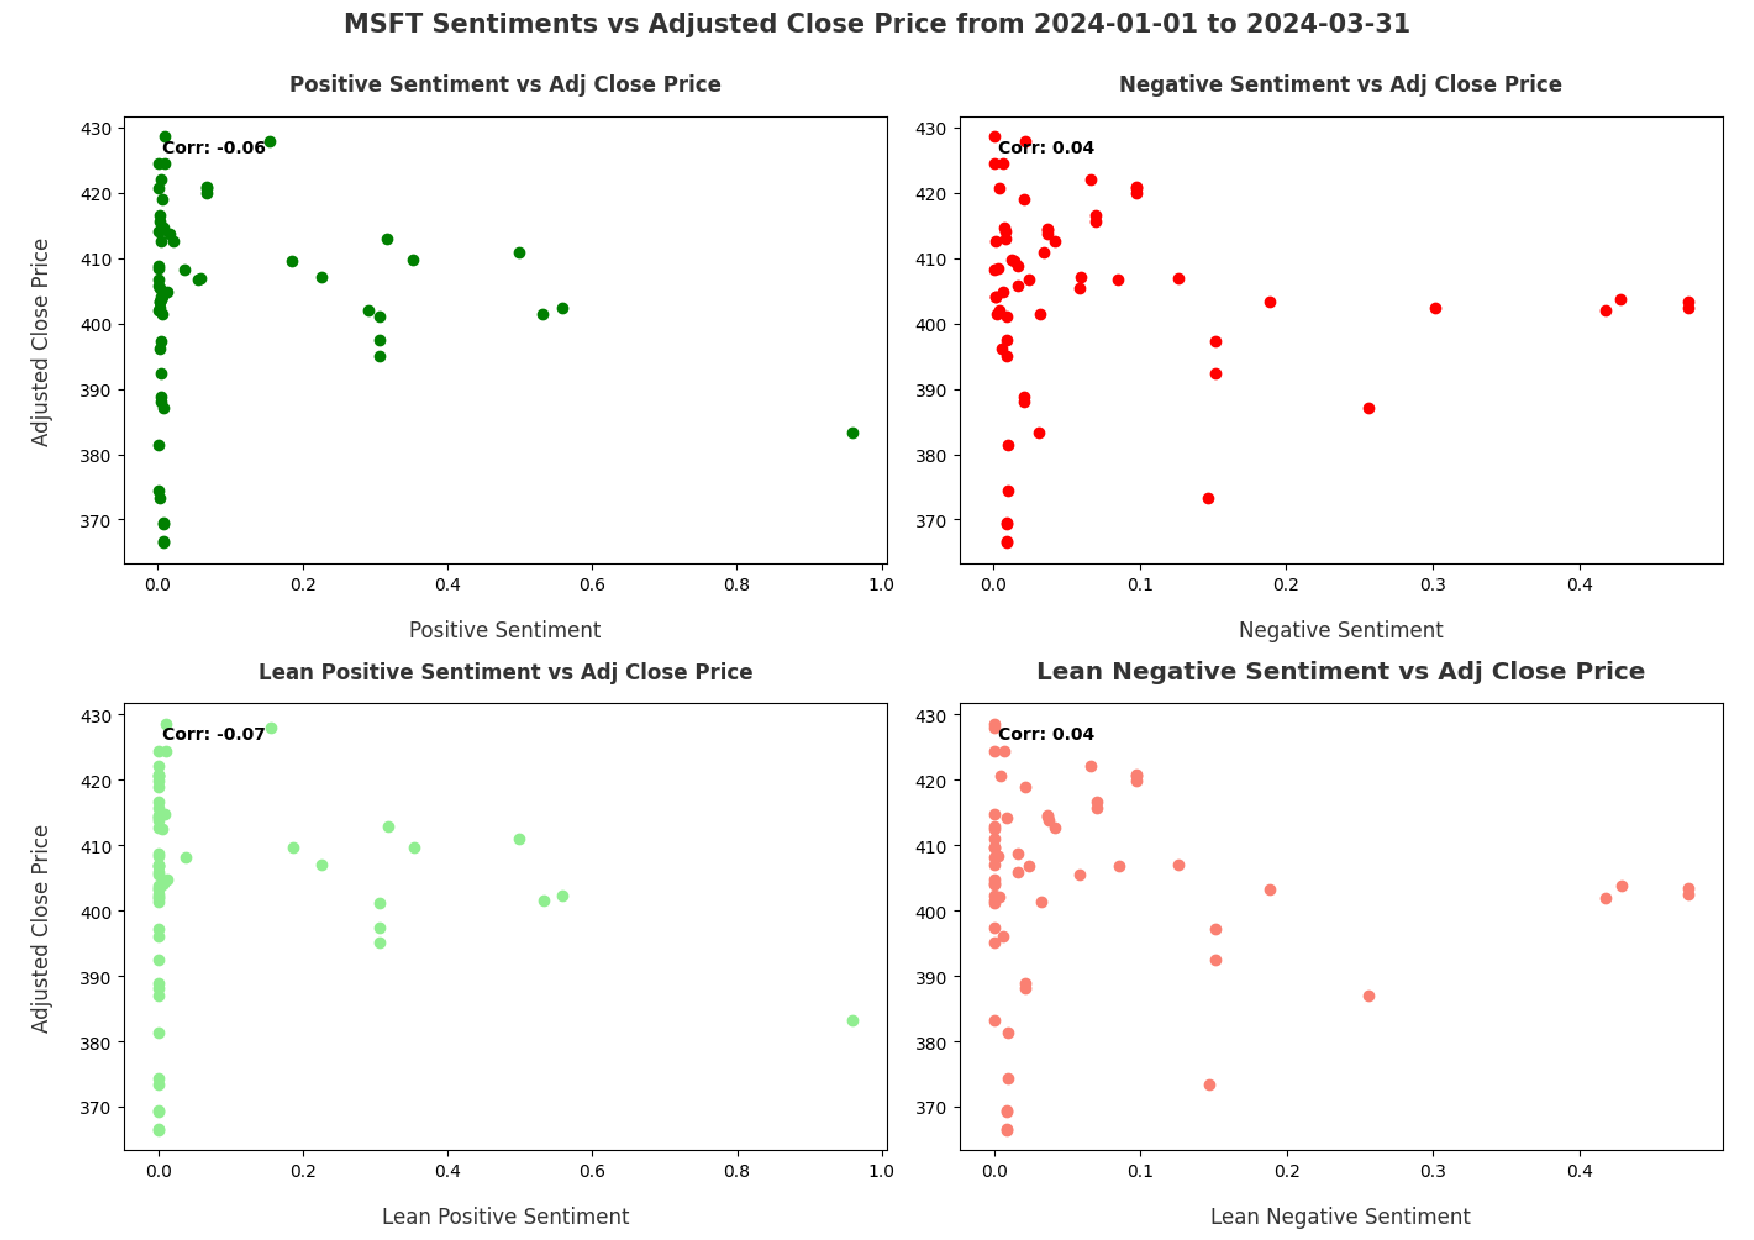
\includegraphics[width=0.9\textwidth]{img/experiment-stock/msft-corr-a.pdf}
  \caption{Microsoft Corp. (MSFT) sentiment correlation with adjusted close price in the first quarter of 2024.}
  \label{fig:elsa-experiment-stock-msft-corr}
\end{figure}

\begin{figure}[ht]
  \centering
  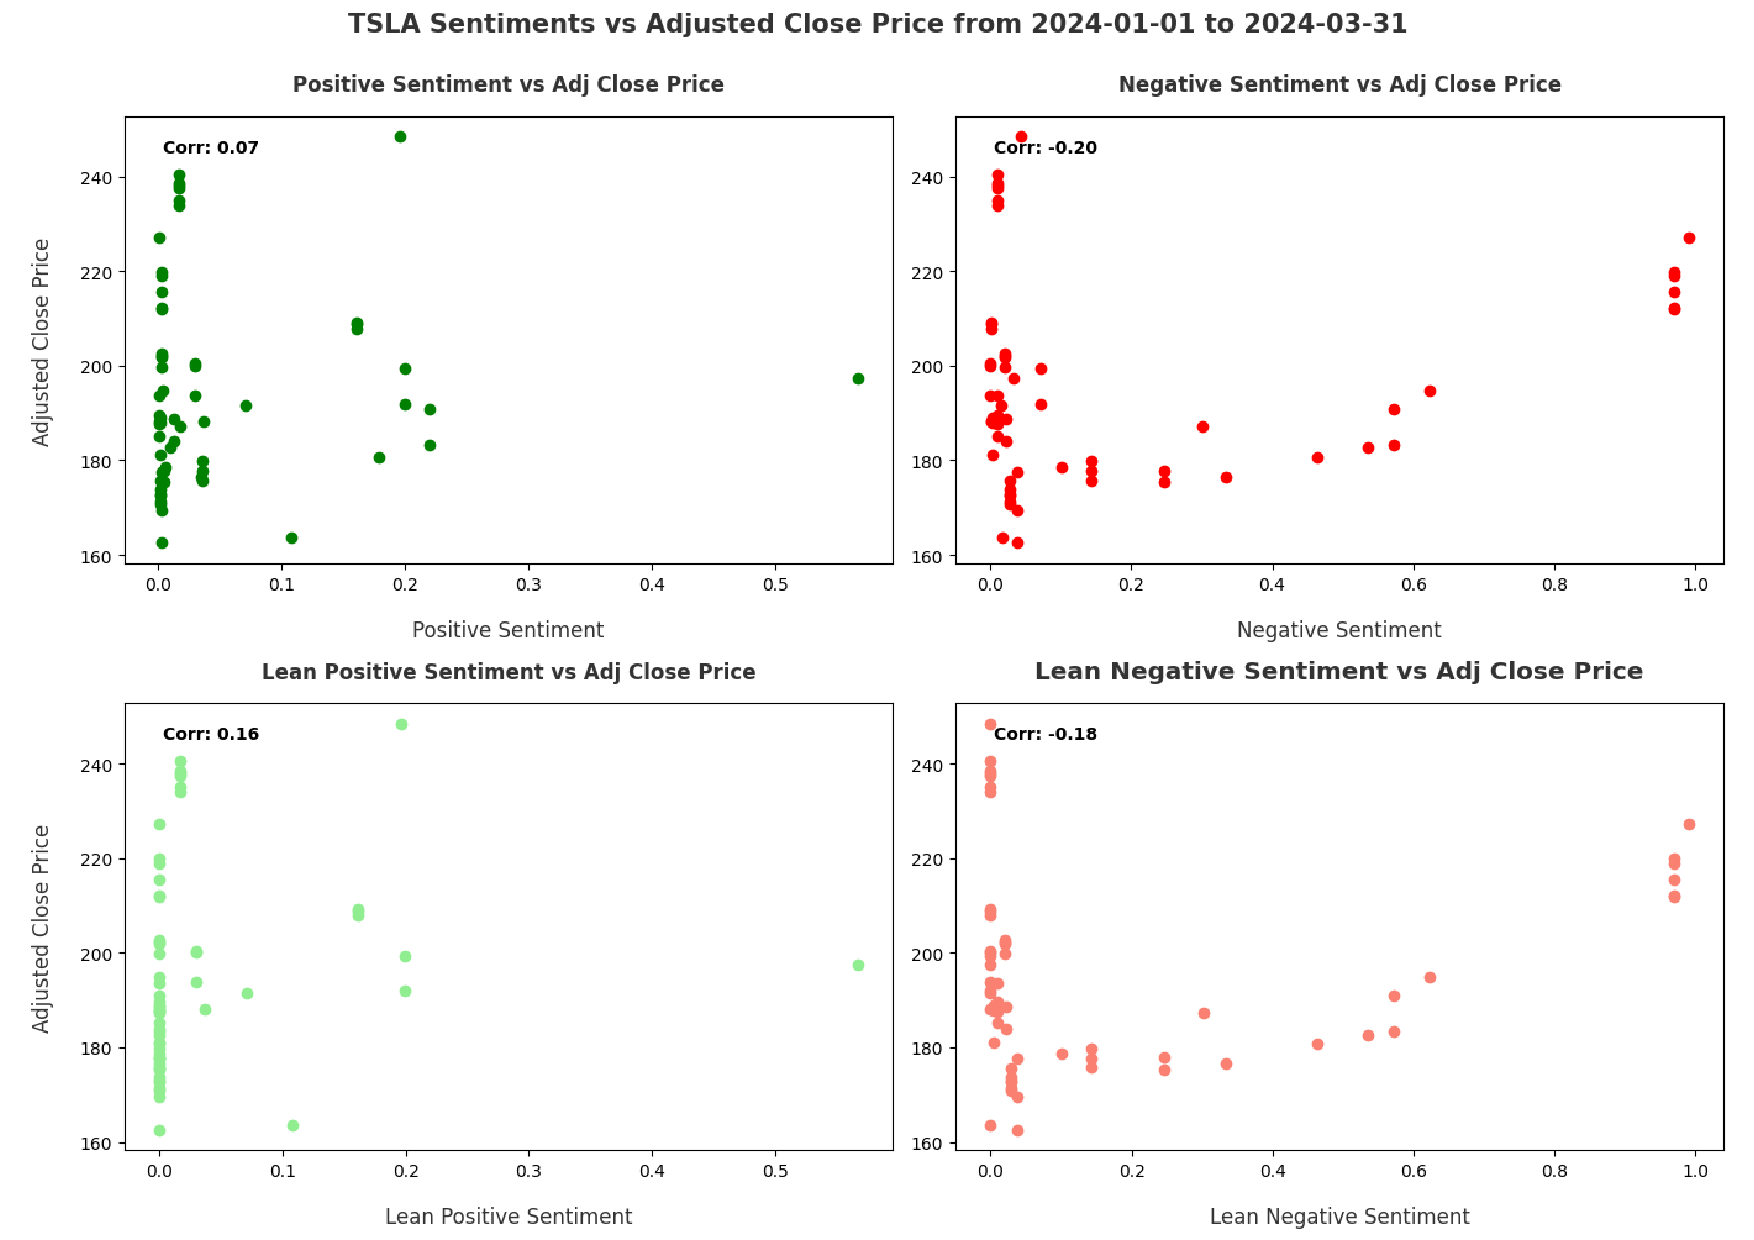
\includegraphics[width=0.9\textwidth]{img/experiment-stock/tsla-corr-a.pdf}
  \caption{Tesla Inc. (TSLA) sentiment correlation with adjusted close price in the first quarter of 2024.}
  \label{fig:elsa-experiment-stock-tsla-corr}
\end{figure}
